\documentclass[a4paper,11pt]{article}

\usepackage[left=2.5cm,top=2.5cm,right=2.5cm]{geometry}

\usepackage{graphicx, subfigure}
\usepackage{longtable}
\usepackage{url}
\usepackage{moreverb}
\usepackage{float}
\usepackage{placeins}
\usepackage{cite}

\usepackage{hyperref}
\hypersetup{backref = true, pagebackref = true, colorlinks= true, linkcolor = black, citecolor = black, urlcolor = black}
\usepackage{framed}
\usepackage{color}
\definecolor{lightgray}{rgb}{0.95,0.95,0.95}
\def\FrameCommand{\colorbox{lightgray}}

\usepackage{sistyle}
\SIunitsep{{\;}}
\SIunitspace{{\,}}

\usepackage[Euler]{upgreek}
\newcommand*{\micro}{\ensureupmath{\upmu}}
\newcommand*{\ohm}{\ensureupmath{\upOmega}}

\usepackage[version=3]{mhchem}

\newcommand{\code}[1]{\texttt{#1}}
\newcommand{\cmd}[1]{\texttt{\color{blue}#1}}

\def\figratio{0.7}

\title{SSH-aerosol}
\date{}
\author{SSH-aerosol user manual and test cases}

\begin{document}

\maketitle

\section*{About}

\begin{itemize}
\item[] {\bf Purpose:} introduction to SSH-aerosol and launching simulations
  for test cases. Very basic post-processing is also
  presented. 
\item[] {\bf Authors:} \\Karine Sartelet, \url{karine.sartelet@enpc.fr};\\
  Youngseob Kim, \url{youngseob.kim@enpc.fr};\\ Zhizhao Wang,
  \url{zhizhao.wang@enpc.fr};\\ C\'edric Flageul,
  \url{cedric.flageul@enpc.fr}; \\Florian Couvidat, \url{florian.couvidat@ineris.fr}.
\item[] {\bf SSH-aerosol version:} 1.1
\item[] SSH-aerosol is distributed under the GNU General Public License v3
\item[] Copyright (C) 2020 CEREA (ENPC), INERIS
\end{itemize}

\tableofcontents

\newpage

\section{Introduction}
%\addcontentsline{toc}{section}{Introduction}
The SSH-aerosol model \cite{sartelet20} represents the physico chemical transformation undergone by aerosols in the troposphere. The term aerosol designs here particles with the surrounding gas. SSH-aerosol is designed to be modular and the user can choose the physical and chemical complexity required.
The model is based on the merge of three state-of-the-art models:
\begin{itemize}
\item SCRAM : The Size-Composition Resolved Aerosol Model \cite{zhu2015} that simulates the dynamics and the mixing state of atmospheric particles. It classifies particles by both composition and size, based on a comprehensive combination of all chemical species and their mass-fraction sections. All three main processes involved in aerosol dynamics (coagulation, condensation/evaporation and nucleation) are included.
\item SOAP: The Secondary Organic Aerosol Processor \cite{couvidat2015} is a thermodynamic model that compute the partitioning of organic compounds. It takes into account several processes involved in the formation of organic aerosol (hygroscopicity, absorption into the aqueous phase of particles, non-ideality and phase separation) and computes the formation of organic aerosol either with a classic equilibrium representation (the partitioning of organic compounds is instantaneous) or with a dynamic representation (where the model solves the dynamic of the condensation/evaporation limited by the viscosity of the particle). The dynamic representation was successfully used \cite{kim2019} for the first study with a 3D air quality model on the impact of particle viscosity on SOA formation.
\item H$^2$O: The Hydrophilic/Hydrophobic Organics \cite{couvidat2012} mechanism uses a molecular surrogate approach to represent the myriad of formation of semi-volatile organic compounds formed from the oxidation in the atmosphere of volatile organic compounds. The mechanism was shown to give satisfactory results for SOA formation (for example in \cite{kim2019}).
\end{itemize}

SSH-aerosol is a free software. You can redistribute it and/or modify it under the terms of the GNU General Public License as published by the Free Software Foundation.
\section*{Hardware and software requirement}
SSH-aerosol is written in the programming language FORTRAN and C++. It can run on PC or a cluster with both the gfortran and the GNU gcc compiler and under a Linux system. Intel compiler should also work. If not, please report to  \url{ssh-aerosol-help@liste.enpc.fr}.
Before the compilation, make sure the construction tool: SCONS has already been installed. 
If not you can obtain it through the instruction of the site: \url{http://www.scons.org/wiki/SconsTutorial1}\\

The following external libraries are required:
\begin{itemize}
\item C++ library Blitz++ (\url{https://github.com/blitzpp/blitz})
\item NetCDF library may be required if you have precomputed coagulation repartition coefficients, you can download from the following site:
\url{http://www.unidata.ucar.edu/downloads/netcdf/index.jsp}
\item SWIG (\url{http://www.swig.org/index.php})
\end{itemize}
After all the required software and library are ready, the compilation can be done by typing a simple command: compile, within a terminal under the program main path.

The random access memory (RAM) requirement for a 0D simulation is very small. 


\section{Folder structure}
%\addcontentsline{toc}{section}{Folder structure}

The SSH-aerosol package contains different repertories for source code,  configuration files, input files, output files, and visualisation of outputs.

\subsection{Source code}
The folder {\it{src}} is where all source code files are stored. The main program file is {\it{ssh-aerosol.f90}}.  Besides, there are 2 sub-folders under the {\it{src}} directory: the {\it{scons}} folder contains the files necessary for compiling the program and the include folder contains the source code, which is itself separated in different folders
\begin{itemize}
\item {\it{Module}} contains SCRAM subroutines to model aerosol dynamics
\item {\it{SOAP}} contains SOAP subroutines to model organic aerosol thermodynamic
\item {\it{CHEMISTRY}} contains H$^2$O subroutines to model gas-phase chemistry. These routines are generated from a list of reactions and species specified in the folder {\it{spack}}.
\item {\it{spack}} contains the gas-phase chemical model generator.
\item {\it{AtmoData}} is a tool for data processing in atmospheric sciences.
 \item {\it{RDB}} contains subroutines for size redistribution used in SCRAM.
\item {\it{isorropia\_aec}} contains ISORROPIA subroutines, a well known module for the computation of inorganic thermodynamic equilibrium between gas and aerosol.
\item {\it{INC}} contains include files which define some system parameter variables.
\end {itemize}

\subsection{Input files}
The main configuration file for the program of SSH-aerosol is {\it{namelist.ssh}}. It requires several input data:
\begin{itemize}
\item The list of species and their properties. They are in the repertory {\it{species-list}}. 
\item The initial concentrations and emissions, which are in the repertory {\it{inputs}}.
\item The configuration files are in the repertory {\it{INIT}}.
\end{itemize}

\subsection{Output files}
The simulation results are stored in the folder {\it{results}}. The folder {\it{graph}} contains a few python routines to postprocess the results and display.
During the simulation, five subfolders and a report file are automatically generated/updated in the folder results:

\begin{itemize}
	\item Subfolder {\it{gas}}: this subfolder contains files that record the time variation of gas phase mass concentration ($\mu$g~m$^{-3}$) of each species.
	 The species name (which is defined by the species list) is adopted as the file name (ex.\textit{HNO3.txt}).\\ 
	 In each file, a total of N + 1 rows of data are listed (N represents the number of iterations). The first line in the file records the initial concentration before the simulation, while line i (i = 2, 3,..., N + 1) records the gas phase mass concentration after i-1 time steps in the simulation. All the concentration files files described in the folder results follow the same output format.
	 
	\item Subfolder {\it{aero}}: this subfolder contains files that record the time variation of particulate mass concentration ($\mu$g~m$^{-3}$) of each species in each size section. The file is named after the species name followed by the index of the size section (index = 1, 2,..., N\_sizebin). For example, file \textit{PNO3\_1.txt} notes the time variation of nitrate particulate mass concentration in the first size section.\\ 
	The files that record the time variation of organic particles, inorganic particles, black carbon, dust, PM$_{2.5}$ and PM$_{10}$ mass concentration ($\mu$g~m$^{-3}$) are also located in the subfolder aero, under the name \textit{Organic.txt, Inorganic.txt, Black\_Carbon.txt, Dust.txt, PM2.5.txt} and \textit{PM10.txt}, respectively.

	\item Subfolder {\it{TM}}: this subfolder contains files that record the time variation of total mass concentration ($\mu g/m^3$) and total aerosol mass concentration of all size sections ($\mu$g~m$^{-3}$). The files is named after the aerosol species name, (followed by the name of its gas phase precursor for recording total mass) and followed by '\_TM'.\\ 
	For example, the file 'PSO4\_TM.txt' notes the time variation of sulfate particulate mass concentration, while the file 'PSO4\_SULF\_TM.txt' notes the time variation of the total sulfate concentration in both the gas phase and the particulate phase.
	
	\item Subfolder {\it{number}}: this subfolder contains files that record the time variation of particulate number concentrations ($\#$~m$^3$) of each size section. The file (ex.\textit{NUMBER\_1.txt}) is named after 'NUMBER\_' followed by the index of size section. \\ The file \textit{TNUM.txt} that records the time variation of total number concentration ($\#$~m$^{-3}$) is located in this subfolder as well.
	
	\item Subfolder {\it{diameter}}: this subfolder contains files that record the time variation of the average diameter ($\mu$m) of each size section. The file (ex.\textit{DIAMETER\_1.txt}) is named after 'DIAMETER\_' followed by the index of size section.
	
	\item Report file {\it{report.txt}}: it records the main settings of the simulation.
\end{itemize}
The user can also modify the name of the output folder ({\it{output\_directory}}) or select the output file type ({\it{output\_type = 1}} for text {\it{outputs and = 2}} for binary outputs) in the file \textit{namelist.ssh}.

\section{Array structure}

The variables and arrays corresponding to the number of compounds in the different
phases, as well as the concentrations are defined in the routine
{\textit{src/Module/ModuleInitialisation.F90}}. Arrays are allocated at the
beginning of the program and desallocated at the end. The array
\textit{concentration\_number} contains the number concentrations for each size
and composition section. \textit{concentration\_mass} contains the mass
concentrations of each chemical compound for each size
and composition section. The order of the chemical compounds is given in the
file \textit{species-list/species-list-aer.dat}. Note that in case of a
viscous aerosol, if several layers are considered, for each organic
compound, the mass concentration is stored for each layer. In that case, for each
size and composition section, the array \textit{concentration\_mass} contains
the mass concentrations of each chemical compound and in each layer if the
compound is organic and hydrophobic. An example of the storage of mass concentrations for a size and composition section $i$ is displayed in Fig.~\ref{fig-array}. In this example, 3 compounds are considered, and three layers are used to represent the condensation/evaporation of the compound~2, which is the only compound hydrophobic and organic out of the 3.

Note that in \textit{soap.cpp}, the organic and aqueous concentrations are stored in different arrays, and a compound can have an aqueous and an organic phase. The organic-phase concentrations in the different layers are
noted \textit{Ap\_layer}, while the aqueous-phase concentrations  are
noted \textit{Aaq}. 
In SSH-aerosol v1.0, an organic compound is assumed to be either hydrophylic,
either hydrophobic, and therefore to have either an organic or an aqueous phase. This will be improved in further version by storing for
each compound both the organic and aqueous-phase concentrations.

\begin{figure}[H]
        \begin{center}
                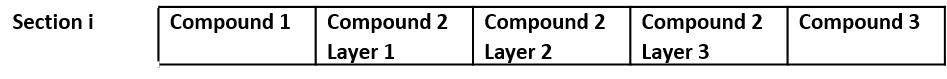
\includegraphics[angle=0,width=0.95\textwidth]{array.png}
        \end{center}
\caption{Storage of the concentrations of chemical compounds in the array {/it{concentration\_mass}} for a section $i$. Case of 3 compounds with 3 layers for compound~2, which is an hydrophobic organic compound.}
\label{fig-array}
\end{figure}

\section{Main options}
%\addcontentsline{toc}{section}{Main options}

The different options are listed in the file {\textit{namelist.ssh}}. They are grouped in different parts.

\subsection{Meteorology}

Input data concerning latitude (in degrees), longitude (in degrees), Temperature (in Kelvin), Pressure (in Pascal) and Relative Humidity (fraction) are listed in the group setup\_meteo. 

\begin{verbatim}

&setup_meteo
latitude = 48.2,                ! Latitude
longitude = 2.22,               ! Longitude
Temperature = 273.16,    	! Temperature
Pressure = 1.01325e05,         	! Pressure
Relative_Humidity = 0.6	! if 0, compute RH from specific humidity. 
                        ! If not, specify RH value.
/

\end{verbatim}

To take into account variable meteorological input data, an additional input file can be used. An example file is given in \code{inputs/meteo.dat}. This file name should be added in the group {\textit{setup\_meteo}} as follows: 

\begin{verbatim}
Relative_Humidity = 0.6,
meteo_file = "inputs/meteo.dat"
/
\end{verbatim}

\code{meteo.dat} file should include time, temperature, pressure, relative humidity and specific humidity. 
If you don't have relative humidity but specific humidity, you put zero to relative humidity. And if you put non-zero relative humidity, specific humidity is not used. 
Please make sure that meteorological data cover the whole simulation period. To do it, the first Time data should be less or equal to \code{initial\_time} and the last Time data should be greater or equal to \code{final\_time} in the group  {\textit{setup\_time}} (see~\ref{sec:time}).


\begin{verbatim}
Time,Temperature,Pressure,RelativeHumidity,SpecificHumidity
19040400.0,298.00,1.01325e05,0.6,5.33039774746E-3    
19058400.0,298.00,1.01325e05,0.6,5.33039774746E-3
\end{verbatim}


\subsection{Time}\label{sec:time}

The group {\textit{setup\_time}} lists the initial time of the simulation (in seconds from 1$^{st}$ January), the final time (in seconds from 1$^{st}$ January) and the time step output of the simulation (in seconds). This time step corresponds to the time step when concentrations are written in the output files, but also to the time step used for splitting the resolution of gaseous chemistry, aerosol processes and emissions. Note that gaseous chemistry and aerosol processes are then solved with smaller time steps.

\begin{verbatim}
&setup_time
initial_time = 0.0,          ! in seconds from January 1st   
final_time = 43200.0,             
delta_t = 43200.0,                 
time_emis = 0,        	 
/
\end{verbatim}

\subsection{Initial conditions}
 
The group {\textit{initial\_condition}} lists the initial conditions of the simulation. The number of size sections is defined in the variable {\textit{N\_sizebin}}. The variable {\textit{tag\_dbd}} defines whether particle size bounds are either generated in the program by assuming they are equally spaced logarithmically ({\textit{tag\_dbd = 0}}) or whether they are read ({\textit{tag\_dbd = 1}}). If they are read, they need to be specified in the group {\textit{initial\_diam\_distribution}}.
The variable {\textit{tag\_init}} defines whether the particles are internally mixed ({\textit{tag\_init = 0}}) or not ({\textit{tag\_init = 1}}) initially. It needs to be set to 0 in the current model version.
The variable {\textit{with\_init\_num}} defines whether number concentrations are estimated from mass concentrations and diameters of each size section ({\textit{with\_init\_num = 0}}) or whether number concentrations are read ({\textit{with\_init\_num = 1}}).
The variable {\textit{wet\_diam\_estimation}} is equal to 0 if isorropia is called
initially to estimate the liquid water content of particles and the wet
diameter. If {\textit{wet\_diam\_estimation}} is equal to 1, the initial wet diameter is
estimated from the input water concentrations (and so it is equal to the dry
diameter if water concentration is zero initially).
Finally, the names of the files containing initial gas and mass concentrations and number concentrations (if {\textit{with\_init\_num = 1}}) are specified by the variables {\textit{init\_gas\_conc\_file}}, {\textit{init\_aero\_conc\_mass\_file}} and {\textit{init\_num\_conc\_num\_file}} respectively.
The unit for gas and aerosol mass concentrations is $\mu$g~m$^{-3}$, and the unit for number concentration is \#particles~m$^{-3}$.

\begin{verbatim}
&initial_condition
with_init_num = 1,        ! 0 estimated from mass and diameter; 
			  ! 1 number conc. for each bin is read 
tag_init = 0,             ! initial method for aerosol species 
                          ! (0 internally mixed,
                          ! 1 mixing_state resolved (notavailable)
wet_diam_estimation = 1   ! Initial estimation of wet diameter
                          ! (0 = isorropia, 1=none)
tag_dbd = 1,	          ! Method for defining particle size bounds 
		          ! (0 if they are auto generated, 1 if bounds are read)
N_sizebin = 50,           ! Number of size bin
init_gas_conc_file = "inputs/init_gas.dat",        ! Initial data for gas
init_aero_conc_mass_file = "inputs/init_aero.dat", ! Initial data for aero mass  
init_aero_conc_num_file = "inputs/init_num.dat",   ! Initial data for aero number  
/

&initial_diam_distribution       
diam_input = 1.0000000000000000E-03	1.2022644346174130E-03	
	1.4454397707459280E-03	1.7378008287493760E-03	2.0892961308540399E-03	
	2.5118864315095799E-03	3.0199517204020170E-03	3.6307805477010140E-03	
	4.3651583224016601E-03	5.2480746024977272E-03	6.3095734448019337E-03	
	7.5857757502918377E-03	9.1201083935590985E-03	1.0964781961431851E-02	
	1.3182567385564069E-02	1.5848931924611141E-02	1.9054607179632480E-02	
	2.2908676527677741E-02	2.7542287033381681E-02	3.3113112148259113E-02	
	3.9810717055349727E-02	4.7863009232263859E-02	5.7543993733715687E-02	
	6.9183097091893658E-02	8.3176377110267125E-02	1.0000000000000001E-01	
	1.2022644346174140E-01	1.4454397707459279E-01	1.7378008287493751E-01	
	2.0892961308540400E-01	2.5118864315095812E-01	3.0199517204020171E-01	
	3.6307805477010152E-01	4.3651583224016621E-01	5.2480746024977298E-01	
	6.3095734448019380E-01	7.5857757502918444E-01	9.1201083935590987E-01	
	1.0964781961431860E+00	1.3182567385564070E+00	1.5848931924611140E+00	
	1.9054607179632490E+00	2.2908676527677749E+00	2.7542287033381689E+00	
	3.3113112148259121E+00	3.9810717055349771E+00	4.7863009232263849E+00	
	5.7543993733715766E+00	6.9183097091893693E+00	8.3176377110267090E+00	
	1.0000000000000011E+01
/ 
\end{verbatim}


\subsection{Mixing state}

The group {\textit{mixing\_state}} defines the mixing state of particles. The variable {\textit{tag\_external}} is set to 0 for internally-mixed particles and to 1 for mixing-state resolved particles. The variable {\textit{N\_groups}} defines the number of group of aerosol compounds for which the composition is discretised. It is set to 1 for internal mixing, because the composition of compounds is then not discretised. In case of mixing-state resolved particles, the belonging of each compound to a group is specified in the input file detailing the aerosol compounds and their properties.
The variable {\textit{N\_frac}} determines the number of mass fraction sections used in the discretisation of composition. 
Finally, the variable {\textit{kind\_composition}} determines whether the fraction are discretized by the program (they are then evenly discretised, {\textit{kind\_composition = 1}}), or whether they are read. If they are read, they need to be specified in the group {\textit{fraction\_distribution}}.


\begin{verbatim}
&mixing_state
tag_external = 0,     ! Mixing state(0 for internally mixed, 
	              ! 1 for mixing-state resolved) 
N_groups = 1,         ! Nb of species groups
N_frac = 1, 	      ! Nb of mass fraction sections
kind_composition = 1, ! Fraction discretization methods 
		      ! (1 for auto discretization and 
                      ! 0 for manual discretization)
/


&fraction_distribution
frac_input= 0.0 1.0,  ! Set fraction bounds manully
/

\end{verbatim}

\subsection{Gas and aerosol species}

The gas phase species are detailed in the group {\textit{gas\_phase\_species}}, where the variable {\textit{species\_list\_file}} contains the name of the file with the list of gas-phase species.
In this file, gas-phase species are listed together with their molar weight in g/mol. Note that the order of the species in this file should not be changed. It is set by the preprocessor of gas-phase chemical schemes.


\begin{verbatim}
&gas_phase_species
species_list_file = "./species-list/species-list-cb05.dat"   
/
\end{verbatim}

Aerosol species are detailed in the group {\textit{aerosol\_species}}, where the variable {\textit{aerosol\_species\_list\_file}} contains the name of the file with the list of aerosol species.
In this file, each aerosol species is listed on a line, together with specific properties: the group to which the species belong in case of mixing-state resolved particles, their molar weight (g/mol) and gaseous precursors, the collision factor, molecular diameter (Angstrom), surface tension (N/m), accomodation coefficient (between 0 and 1), density in $\mu$g~$\mu$m$^3$ and whether or not the species is non-volatile ("1" for condensable but low-volatility species and "0" for others).
Note that the condensation of non-volatile species is solved dynamically.
The categories to which species correspond are also listed. They should not be modified and they must correspond to those set in the routine {\textit{ModuleInitialisation.f90}} of SSH-aerosol.

\begin{verbatim}
&aerosol_species
aerosol_species_list_file = "./species-list/species-list-aer.dat",
/
\end{verbatim}

Particles can be made of dust (PMD), black carbon (PBC), sulfate (PSO4), nitrate (PNO3), ammonium (PNH4), chloride (PCL), sodium (PNA) and organics. Characteritics of the surrogates for aerosol organic species are detailed in Table~\ref{species} and Table~\ref{speciesb}.

\begin{footnotesize}
\begin{table}
\caption{Characteristic of the surrogates for aerosol organic species: abbreviation of the surrogate, type 	
	(A: hydrophilic, type B: hydrophobic, type C: hydrophobic non-volatile and not used to compute activity coefficients),
	Molecular structure, Molecular weight MW (g.mol$^{-1}$), OM/OC ratio r, Henry's law constant H ($\times$ 10$^8$ M/atm), partitioning constant K$_p$
(m$^3$~$\mu$g$^{-1}$) for an ideal organic phase of molar mass 200 g/mol at 298~K, Enthalpy of vaporization (kJ.mol$^{-1}$), and precursors. The abbreviation n.v. means non volatile.}
\centering
\begin{tabular}{|c|c|p{3.8cm}|c|c|c|c|c|c|c}
\hline
	Surrogate & Type & Molecular structure& MW & r & H  & K$_p$ & $\Delta$H$_{\mathrm{vap}}$ & Precursor \\
\hline
	BiMT & A & methyl tetrol & 136 & 2.3 & 330 & 0.064 & 38 &  \\
	BiPER & A & methyl dihydroxy dihydroperoxide & 168 & 2.8 & 81 & 0.036 & 38 &  \\
	BiDER & A & methyl tetrol & 136 & 2.3 & 891 & 0.227 & 38 & isoprene \\
	BiMGA & A & methyl glyceric acid (MGA) & 120 & 2.5 & 5.3 & 0.007 & 43 & \\
	BiNGA & B & nitrate derivative of MGA & 165 & 3.5 & 0.4 & 0.007 & 43 & \\
	BiNIT3 & B & methyl hydroxy trinitrate butane & 272 & 4.6 & 0.4 & 0.064 & 38 &  \\
\hline
	BiA0D & A & pinonaldehyde & 168 & 1.4 & 0.02 & 0.0003 & 50 & \\
	BiA1D & A & norpinic acid & 170 & 1.5 & 1.12 & 0.428 & 50 & mono- \\
	BiA2D & A & pinic acid & 186 & 1.7 & 2.7 & 0.650 & 109 & terpenes\\
	BiA3D & B & 3-methyl-1,2,3-butane tricarboxylic acid & 204 & 2.1  & - & n.v. & - &\\
	BiNIT & B & Nitrooxy-limonene-ol & 215 & 1.8 & 0.02 & 0.037 & 50 & \\
	Monomer & C & C$_{10}$H$_{14}$O$_9$ & 278 & 2.3 & - & n. v. & - &\\
	Dimer & C & C$_{19}$H$_{28}$O$_{11}$ & 432 & 1.9 & - & n. v. & - & \\
\hline
	BiBlP & B & C15 hydroxy nitrate aldehyde & 298 & 1.7 & 2.34 & 154.9 & 175 & sesqui- \\
	BiBmP & B & C15 oxo aldehyde & 236 &1.3 & - & 0.309 & 175 & terpenes \\ 
\hline
	AnBlP & B & methyl nitro benzoic acid & 167 & 2 & 2.48 & 1.37 & 50 &     xylenes\\
	AnBmP & B & methyl hydroxy benzoic acid & 152 & 1.6 & 12.4 & 0.011 & 50 & and\\
	AnClP & C & No structure & 167 & 2 & - & n. v. & - & toluene\\
\end{tabular}
\label{species}
\end{table}


\begin{table}
\caption{Characteristic of the surrogates for aerosol organic species: abbreviation of the surrogate, type 	
	(A: hydrophilic, type B: hydrophobic, type C: hydrophobic non-volatile and not used to compute activity coefficients),
	Molecular structure, Molecular weight MW (g.mol$^{-1}$), OM/OC ratio r, Henry's law constant H ($\times$ 10$^8$ M/atm), partitioning constant K$_p$
(m$^3$~$\mu$g$^{-1}$) for an ideal organic phase of molar mass 200 g/mol at 298~K, Enthalpy of vaporization (kJ.mol$^{-1}$), and precursors. The abbreviation n.v. means non volatile.}
\centering
\begin{tabular}{|c|c|p{3.8cm}|c|c|c|c|c|c|c}
\hline
	Surrogate & Type & Molecular structure& MW & r & H  & K$_p$ & $\Delta$H$_{\mathrm{vap}}$ & Precursor \\
\hline
	ACIDMAL& A & maleylacetic acid & 158& 2.2 & 8685 & 2.02 & 50 & phenol\\
	       &   &                   &    &     &                         &      &       & catechol\\
	       &   &                   &    &     &                         &      &       & benzene\\
\hline
	DHMB & A & dihydroxymethyl & 154 & 1.8 & 36.2 & 0.026 & 50 & methyl- \\
	     &   &  benzoquinone   &     &      &                        &       &       &  catechol \\
	     &   &     &     &      &                        &       &       &  cresol \\
\hline
	PSYR  &A & C$_{8}$H$_{10}$O$_{5}$& 186 & 1.9 & 14.5  & 0.0123  & 50 & syringol \\
\hline
	GHDPerox &A &  SOA (hydroperoxide) & 174 &2.1 & 63.3 & 0.171 & 50 & guaiacol \\
\hline
	PAHlN & A & dihydroxytere &198& 2.1 & n. v.  & - & - & naphtalene \\
	      &   & phtalic acid                  &   &      &                           &               &   &  methyl- \\
	PAHhN & A & phthalic acid & 166 & 1.7 & 14.9 & 0.093 & 50 & naphtalene\\
\hline
	POAlP & B & primary OA of low volatility & 280 & 1.3 & - & 1.1 & 106 & -    \\
	POAmP & B & primary OA of medium volatility & 280 & 1.3 & - & 0.0116 & 91 & -  \\
	POAhP & B & primary OA of high volatility & 280 & 1.3  & - & 0.00031 & 79 & -  \\
	SOAlP & C & secondary OA of low volatility & 392 & 1.8 & - &  110 & 106 & POAlP    \\
	SOAmP & B & secondary OA of medium volatility & 392 & 1.8 & - & 1.16 & 91 & POAmP   \\
	SOAhP & B & secondary OA of high volatility & 392 & 1.8 & - & 0.031 &79 & POAhP  \\
\end{tabular}
\label{speciesb}
\end{table}


\end{footnotesize}


\subsection{Emissions}

The group {\textit{emissions}} defines options linked to emissions. The variable {\textit{tag\_emis}} defines whether emissions are used ({\textit{tag\_emis = 1}}) or not ({\textit{tag\_emis = 0}}).
Emissions are assumed to be internally mixed. Gas-phase emissions and/or particle-phase emissions can be specified. Number concentrations at emission may be determined from mass emissions and section diameters if the variable {\textit{with\_emis\_num}} is set to 0. They are read from a file is the variable {\textit{with\_emis\_num}} is set to 1. 
The name of the file containing the list of gas-phase emitted species and their emission rates should be specified using the variable {\textit{emis\_gas\_file}}. Similarly, the name of the file containing the list of aerosol-phase emitted species and their emission rates should be specified using the variable {\textit{emis\_aero\_mass\_file}}. Note that the unit for emission rates is $\mu$g~m$^{-3}$~s$^{-1}$. If number emissions are read, the name of the files containing emission rates should be specified using the variable {\textit{emis\_aero\_num\_file}}. The units of number emissions should be \#particles~m$^{-3}$~s$^{-1}$.

\begin{verbatim}
&emissions
tag_emis = 0,       ! 0 Without emissions, 
                    ! 1 with internally-mixed emissions, 
                    ! 2 with externally-mixed emissions  
with_emis_num = 0,  ! 0 if number estimated from mass and diameter; 
		    ! 1 if read
emis_gas_file = "./inputs/emis_gas.dat",
emis_aero_mass_file = "./inputs/emis_aero.dat", 
emis_aero_num_file = "./inputs/emis_aero_num.dat" 
/
\end{verbatim}


\subsection{Numerical and physical options}

\subsubsection{Gas-phase chemistry}

The group {\textit{physic\_gas\_chemistry}} lists options related to gas-phase chemistry. 
The variable {\textit{tag\_chem}} defines whether gas-phase chemistry is used ({\textit{tag\_chem = 1}}) or not ({\textit{tag\_chem =0}}). 
Photolysis reactions may be taken into account ({\textit{with\_photolysis = 1}}) or ignored ({\textit{with\_photolysis = 0}}). In case photolysis reactions are taken into account, they may be attenuated by clouds. The cloud attenuation (variable attenuation) has a value below 1 in case of cloud attenuation of photolysis, and it is equal to 1 if no cloud attenuation (clear sky).
Heterogeneous reactions at the surface of particles may be taken into account (variable {\textit{with\_heterogeneous = 1}}) or ignored (variable {\textit{with\_heterogeneous = 0}}). An adaptive time step may be used to solve gaseous chemistry (variable {\textit{with\_adaptive}}). It is advised to use the adaptative time step and to set the relative tolerance to decide if the time step is kept to 0.01 or 0.001. The minimum time step (in seconds) that can be used in the solver is set with the variable {\textit{min\_adaptive\_time\_step}}.


\begin{verbatim}
&physic_gas_chemistry
tag_chem = 0,		   	 ! Tag of gas-phase chemistry
attenuation = 1.d0,              ! Cloud attenuation field (0 to 1)
				 ! (1 = no attenuation)
option_photolysis = 1,	 	 ! 1 if default photolysis rates, 
                                 ! 2 if read from binary files.
time_update_photolysis = 100000. ! if photolysis are read, 
				 ! time in seconds between two reads
with_heterogeneous = 0,          ! Tag of heterogeneous reaction 
with_adaptive = 1,               ! Tag of adaptive time step for chemistry 
				 ! 1 if adaptive time step.
adaptive_time_step_tolerance = 0.001, ! Relative tolerance to decide 
			 	 ! if the time step is kept
min_adaptive_time_step = 0.001,  ! Minimum time step in seconds
photolysis_dir = "./photolysis/", ! Directory where binary files are.
photolysis_file = "./photolysis/photolysis-cb05.dat",  ! Photolysis list
n_time_angle = 9,                ! Parameters specific to the tabulation 
			 	 ! of photolysis rates
time_angle_min = 0.d0,   ! if read from files
delta_time_angle = 1.d0,
n_latitude = 10,
latitude_min = 0.d0,
delta_latitude = 10.d0,
n_altitude = 9,
altitude_photolysis_input = 0.0, 1000.0, 2000.0, 3000.0, 4000.0, 5000.0, 
	10000.0, 15000.0, 20000.0, 
/
\end{verbatim}


\subsubsection{Numerical issues related to aerosols}

The group {\textit{physic\_particle\_numerical\_issues}} lists options related to numerical issues when solving aerosol dynamics. 
The variable {\textit{DTAEROMIN}} specifies the The minimum time step (in seconds) that can be used in the solver. 
Different redistribution methods of mass and number concentrations onto the fixed diameter grids may be used (variable {\textit{redistribution\_method}}). If only the process of condensation/evaporation is considered for aerosol dynamics, then it is possible to not apply redistribution ({\textit{redistribution\_method = 0}}). If nucleation and/or coagulation is also considered, then a redistribution method should be chosen. It is advised to use the redistribution 10 (moving diameter) or 12 (Euler coupled). The different redistributions ({\textit{redistribution\_method}}) are Euler mass (3), Euler number (4), hemen (5), moving diameter (10), area-based as in SIREAM (11), Euler coupled (12).
The density of particles may be computed during the simulation depending on the composition of particles if the variable {\textit{with\_fixed\_density}} is set to 0. If it is set to 1, then the density is fixed through the simulation to the value set by the variable {\textit{fixed\_density}} (in $\mu$g~$\mu$m$^{-3}$). Note that the variable {\textit{fixed\_density}} needs to be set.

Numerically, the nucleation and condensation/evaporation of inorganics are always solved simultaneously, because nucleation and condensation/evaporation are competing processes. Coagulation may also be coupled to nucleation and condensation/evaporation if the variable splitting is set to 1. If splitting = 0, coagulation is splitted from nucleation and condensation/evaporation. If nucleation is taken into account, it is recommended to set splitting to 1.

\begin{verbatim}
&physic_particle_numerical_issues
DTAEROMIN = 1E-5,              	! Minimum time step
redistribution_method = 0,   	! Redistibution method: 0: no redistribution
				! 10: 10 Moving Diameter, 12: euler_coupled
with_fixed_density = 1,       	! 1 if density is fixed - 0 else
fixed_density = 1.84D-06,        
splitting = 0,             ! 0 if coagulation and 
		! (condensation/evaporation+nucleation) are splitted 
		! 1 if they are not
/
\end{verbatim}

\subsubsection{Coagulation}

The group {\textit{physic\_coagulation}} lists options related to coagulation. The variable {\textit{with\_coag}} defines whether coagulation is taken into account ({\textit{with\_coag = 1}}) or not ({\textit{with\_coag =0}}). 
Repartition coefficients may be computed in the simulation ({\textit{i\_compute\_repart = 1}}) or read from a netcdf file ({\textit{i\_compute\_repart = 0}}). If they are read from a file, its name should be specified ({\textit{Coefficient\_file}}). If they are computed, the number of Monte Carlo points used to compute them should be specified ({\textit{Nmc}}). This number should be large enough and its value depends on the section discretisation used.


\begin{verbatim}
&physic_coagulation
with_coag = 1,                 ! Tag of coagulation
i_compute_repart = 1,          ! 0 if repartition coeff are not computed 
                               ! but read from file, 1 if they are 
i_write_repart = 0,            ! 1 to write repartition coeff file, 0 otherwise
Coefficient_file = "coef_s1_f1_b6.nc",  ! Repartition coefficient file
Nmc = 2000                     ! Number of Monte Carlo points to compute
                               ! repartition coefficients
/
\end{verbatim}
          
\subsubsection{Condensation/evaporation}

The group {\textit{physic\_condensation}} lists options related to condensation/evaporation. The variable {\textit{with\_cond}} defines whether condensation/evaporation is taken into account ({\textit{with\_cond = 1}}) or not ({\textit{with\_cond =0}}). Kelvin effect may be taken into account ({\textit{with\_kelvin\_effect = 1}}), as recommended if ultrafine particles are simulated, or ignored ({\textit{with\_kelvin\_effect = 0}}).
For the condensation/evaporation of inorganic compounds, {\textit{Cut\_dim}} corresponds to the diameter under which thermodynamic equilibrium is assumed. Set it to 0 to compute dynamically condensation/evaporation for all particles, and set it to a value larger than larger diameter to assume thermodynamic equilibrium.
For the condensation/evaporation of organic compounds, ISOAPDYN determines whether thermodynamic equilibrium is assumed for all particles ({\textit{ISOAPDYN = 0}}) or whether condensation/evaporation is computed dynamically ({\textit{ISOAPDYN = 1}}). Even if it is computed dynamically, thermodynamic equilibrium may be used for the condensation/evaporation of small particles by setting a characteristic time under which equilibrium is assumed for organics (e.g. {\textit{tequilibrium}} = 0.1 seconds). For numerical reasons, {\textit{tequilibrium}} may not be set to 0, but condensation/evaporation of all particles is solved dynamically if ({\textit{ISOAPDYN = 1}}) and {\textit{tequilibrium}} is set to a small value (e.g. 1.d-15). In the current version of the code, the diffusion coefficient {\textit{dorg}} in the organic phase is assumed constant. Typical values would be 1.d-12 for non viscous particles and 1.d-24 for very viscous particles. 
The variable {\textit{coupled\_phases}} should be set to 1 if the resolution of the aqueous and organic phases is coupled and to 0 if they are solved independently. The interactions between compounds in the particles may be assumed to be ideal ({\textit{activity\_model = 1}}), or activity coefficients may be computed with unifac (interactions between organics only, {\textit{activity\_model = 2}}) or with aiomfac ({\textit{activity\_model = 3}}).

\begin{verbatim}
&physic_condensation
with_cond = 0,             ! Tag of condensation/evaporation
Cut_dim = 0.0,             ! Diameter under which equilibrium
                           ! is assumed for inorganics
ISOAPDYN = 1,              ! 0 = equilibrium, 1 = dynamic
nlayer = 1,
with_kelvin_effect = 0,    ! 1 if kelvin effect is taken into account.
tequilibrium = 0.1,        ! time under which equilibrium 
                           ! is assumed for organics.
dorg = 1.d-12,             ! diffusion coefficient 
                           ! in the organic phase.
coupled_phases = 1,        ! 1 if aqueous and organic phases 
                           ! are coupled
activity_model = 1,        ! 1: ideal, 2: unifac, 3: aiomfac
epser = 0.01,              ! relative error for time step adjustment
epser_soap = 0.01,         ! relative difference of ros2 in SOAP  
/

\end{verbatim}

\subsubsection{Nucleation}


The group {\textit{physic\_nucleation}} lists options related to nucleation. The variable {\textit{with\_nucl}} defines whether nucleation is taken into account ({\textit{with\_nucl = 1}}) or not ({\textit{with\_nucl =0}}). If nucleation is taken into account, then the lower diameter bound should be about 1~nm. Three nucleation models are implemented.
\begin{itemize}
\item binary: water and sulfate with the parameterisation of \cite{vehk} ({\textit{nucl\_model = 0}})
\item ternary: water, sulfate and ammonium with the parameterisation of \cite{napari} ({\textit{nucl\_model = 1}}) or with the parameterisation of \cite{merikantoa, merikantob} ({\textit{nucl\_model = 2}}).
To avoid artificially large nucleation rates in the parameterisation of \cite{napari}, a maximum nucleation rate of 1.d6 \#particles~cm$^{-3}$ is set.
\end{itemize}


\begin{verbatim}
&physic_nucleation
with_nucl = 0,    ! Tag of nucleation 
	    	  ! Need to have the lowest diameter about 1 nm.
nucl_model = 0,   ! Nucleation model 
                  ! (0: binary of Vekhamaki, 1: ternary of Napari, 
		  ! 2: ternary of Merikanto)
/
\end{verbatim} 

\subsubsection{Organics}

Concerning organic reactions in the particles, oligomerization of pinonaldehyde may be considered ({\textit{with\_oligomerization = 1}}) or not.


\begin{verbatim}
&physic_organic
with_oligomerization = 1      
/
\end{verbatim}


\subsection{Output}

The output directory may be specified, as well as the format of the files (text if {\textit{output\_type = 1}}, and binary if {\textit{output\_type = 2}}).
 
\begin{verbatim}
&output
output_directory = "results/coag/", 
output_type = 1               ! 1: text, 2: binary
/
\end{verbatim}

\subsection{Coupling with external tools}

SSH-aerosol can be coupled with external (3D) tools using the shared library (\texttt{libssh-aerosol.so}) available in the \texttt{src} folder after compilation.
The \texttt{.so} file is produced with the command \texttt{./compile --sharedlib=yes}.
A prototype of the typical workflow is described hereafter.

\subsubsection*{Prerequisite}

The following piece of \textbf{C} code is taken from the open-source CFD code Code\_Saturne.
The subroutine \texttt{\_get\_dl\_function\_pointer} is used to interact with the members of the shared library object.

\begin{verbatim}
/*----------------------------------------------------------------------------
 * Get a shared library function pointer
 *
 * parameters:
 *   handle           <-- pointer to shared library (result of dlopen)
 *   name             <-- name of function symbol in library
 *   errors_are_fatal <-- abort if true, silently ignore if false
 *
 * returns:
 *   pointer to function in shared library
 *----------------------------------------------------------------------------*/

static void *
_get_dl_function_pointer(void        *handle,
                         const char  *lib_path,
                         const char  *name,
                         bool         errors_are_fatal)
{
  void  *retval = NULL;
  char  *error = NULL;

  dlerror();    /* Clear any existing error */

  retval = dlsym(handle, name);
  error = dlerror();

  if (error != NULL) { /* Try different symbol names */
    char *name_ = NULL;
    dlerror();    /* Clear any existing error */
    int _size_ = strlen(name) + strlen("_");
    BFT_MALLOC(name_, _size_ + 1, char);
    strcpy(name_, name);
    strcat(name_, "_");
    retval = dlsym(handle, name_);
    error = dlerror();
    BFT_FREE(name_);
  }

  if (error != NULL && errors_are_fatal)
    bft_error(__FILE__, __LINE__, 0,
              _("Error while trying to find symbol %s in lib %s: %s\n"),
              name,
              lib_path,
              dlerror());

  return retval;
}
\end{verbatim}

\subsubsection*{Initialisation}

First, the external code should load the shared library using \texttt{dlopen}.
\begin{verbatim}
  /* Load the shared object */
  _aerosol_so = dlopen(lib_path, RTLD_LAZY);
\end{verbatim}

Then, it should decide whether SSH-aerosol outputs to the terminal or to a file.
\begin{verbatim}
  /* Declare SSH-aerosol as not running standalone */
  {
    typedef void (*cs_set_sshaerosol_t)(bool*);
    cs_set_sshaerosol_t fct =
      (cs_set_sshaerosol_t) _get_dl_function_pointer(_aerosol_so,
                                        lib_path,
                                        "api_set_sshaerosol_standalone",
                                        true);
    bool flag = false;
    fct(&flag);
  }
  /* Force SSH-aerosol to write output to a file */
  if (cs_glob_rank_id <= 0) {
    typedef void (*cs_set_sshaerosol_t)(bool*);
    cs_set_sshaerosol_t fct =
      (cs_set_sshaerosol_t) _get_dl_function_pointer(_aerosol_so,
                                                     lib_path,
                                                    "api_set_sshaerosol_logger",
                                                     true);
    bool flag = true;
    fct(&flag);
  }
\end{verbatim}

Then, SSH-aerosol can be initialised.
\begin{verbatim}
  /* Initialize SSH-aerosol */
  {
    const char namelist_ssh[40] = "namelist_coag.ssh";
    typedef void (*cs_set_sshaerosol_t)(char*);
    cs_set_sshaerosol_t fct =
      (cs_set_sshaerosol_t) _get_dl_function_pointer(_aerosol_so,
                                                     lib_path,
                                                    "api_sshaerosol_initialize",
                                                     true);
    fct(&namelist_ssh);
  }
\end{verbatim}

\subsection*{Time advancement}

The time advancement in the external 3D code could look as follow: for each time step, a loop on the cells is performed and the code
\begin{itemize}
\item Sets (initialises) the time step in SSH-aerosol using \texttt{api\_set\_sshaerosol\_dt}
\item Sets the Pressure, Temperature, pH, ... in SSH-aerosol using \texttt{api\_set\_sshaerosol\_temperature} and similar functions
\item Sets the gaseous concentrations in SSH-aerosol using \texttt{api\_set\_sshaerosol\_gas\_concentration}
\item Sets the aerosol concentrations in SSH-aerosol using \texttt{api\_set\_sshaerosol\_aero\_concentration}
\item Sets the aerosol numbers in SSH-aerosol using \texttt{api\_set\_sshaerosol\_aero\_number}
\item Advance in time (computes one time step) for the gaseous chemistry and for the aerosol chemistry in the given cell using \texttt{api\_call\_sshaerosol\_gaschemistry} and \\ \texttt{api\_call\_sshaerosol\_aerochemistry}
\item Reads the new concentrations in the given cell from SSH-aerosol using the \texttt{api\_get\_*} functions and use them in the external code
\end{itemize}

\subsection*{Finalisation}

At the end of the simulation, the external tool should call the subroutine \texttt{api\_sshaerosol\_finalize}.
Then, the shared library can  be released using \texttt{dlclose}.
\begin{verbatim}
    dlclose(_aerosol_so);
\end{verbatim}

\subsection*{Parallelism}
If the external tool is running with MPI, each MPI process should load the shared library and perform all the aforementioned operations.
However, please note that only one MPI process can use the logger (\texttt{api\_set\_sshaerosol\_logger}).

\section{Test cases}
%\addcontentsline{toc}{section}{Test cases}

This section presents a few test-cases to demonstrate how the model works.

During the practical session, we will work in the directory
{\textit{ssh-aerosol}}. 
To compile the program, please type {\it{compile}}. Before compiling, you may
clean previous compilation by typing {\it{clean}}.

The main options of the simulations are detailed in the namelist files (for
example {\it{INIT/namefile\_coag.ssh}}), which are in the folder {\it{INIT}}, and
initial conditions (meteorological, gas and aerosol concentrations) are
required.
The simulation can be run by typing {\it{ssh-aerosol INIT/namefile\_coag.ssh}}.

The list of species and parameters are detailed in the files {\it{species-list/species-list-aer.dat}} and {\it{species-list/species-list-cb05.dat}}. The name and location of the files can be modified in the configuration file {\it{namelist*.ssh}}.

Different processes can be considered (set the flag to 1) or ignored (set the flag to 0): emissions (flag {\it{tag\_emis}}),
gaseous chemistry (flag {\it{tag\_chem}}),
coagulation (flag {\it{with\_coag}}),
condensation (flag {\it{with\_cond}}),
nucleation (flag {\it{with\_nucl}}).
Internal mixing (flag {\it{tag\_external}} set to 0) or mixing-state resolved particles (flag {\it{tag\_external}} set to 1) can be considered. 

\subsection{Dynamic of coagulation and condensation}

In the literature, to test the overall behaviour of PM models, the following 
basic tests of
condensation and coagulation of sulfate are often considered \cite{seigneur1986simulation,zhang1999simulation,binkowski2003models}. A tri-modal PM distribution is considered initially,
with particles being made exclusively of sulfate. The parameters of the initial distribution
considered here are those of hazy conditions for the condensation test with a sulphuric
acid production rate of 9.9 $\mu$g m$^{-3}$, and those of urban conditions for the coagulation test \cite{seigneur1986simulation,zhang1999simulation} , because these two tests represent the two most
stringent conditions for coagulation and condensation. Temperature is taken as 283.15 K.
Simulations are conducted for 12 hours.
The reference solutions for the coagulation and condensation tests are those of \cite{zhang1999simulation} obtained with another models.


\subsubsection{Coagulation}
\label{coag-test}

The configuration file for this test is {\it{namelist\_coag.ssh}}.
In the coagulation test case, only coagulation is considered by setting the variable of {\it{with\_coag}} of the file {\it{namelist\_coag.ssh}} to 1.

The partition coefficients may be precomputed in a C++ routine. Here, the
coefficients are directly computed by SSH-aerosol (option {\it{i\_compute\_repart}}), using a
Monte-Carlo method (Nmc represents the Monte Carlo number). The larger Nmc is,
the more accurate the coefficients are, but the more CPU time it takes to
compute them.
Run the simulation by typing {\it{ssh-aerosol INIT/namelist\_coag.ssh}}.
You can compare the number and volume distribution of particles at the initial
time and after 12~h by going to the repertory {\it{graph}} and by running the
python script {\it{dN\_Vdlogd\_coag.py}}.
SSH-aerosol does very well in representing the growth of particles by
coagulation, as shown in Fig~\ref{fig-coag}.

\begin{figure}[H]
        \begin{center}
                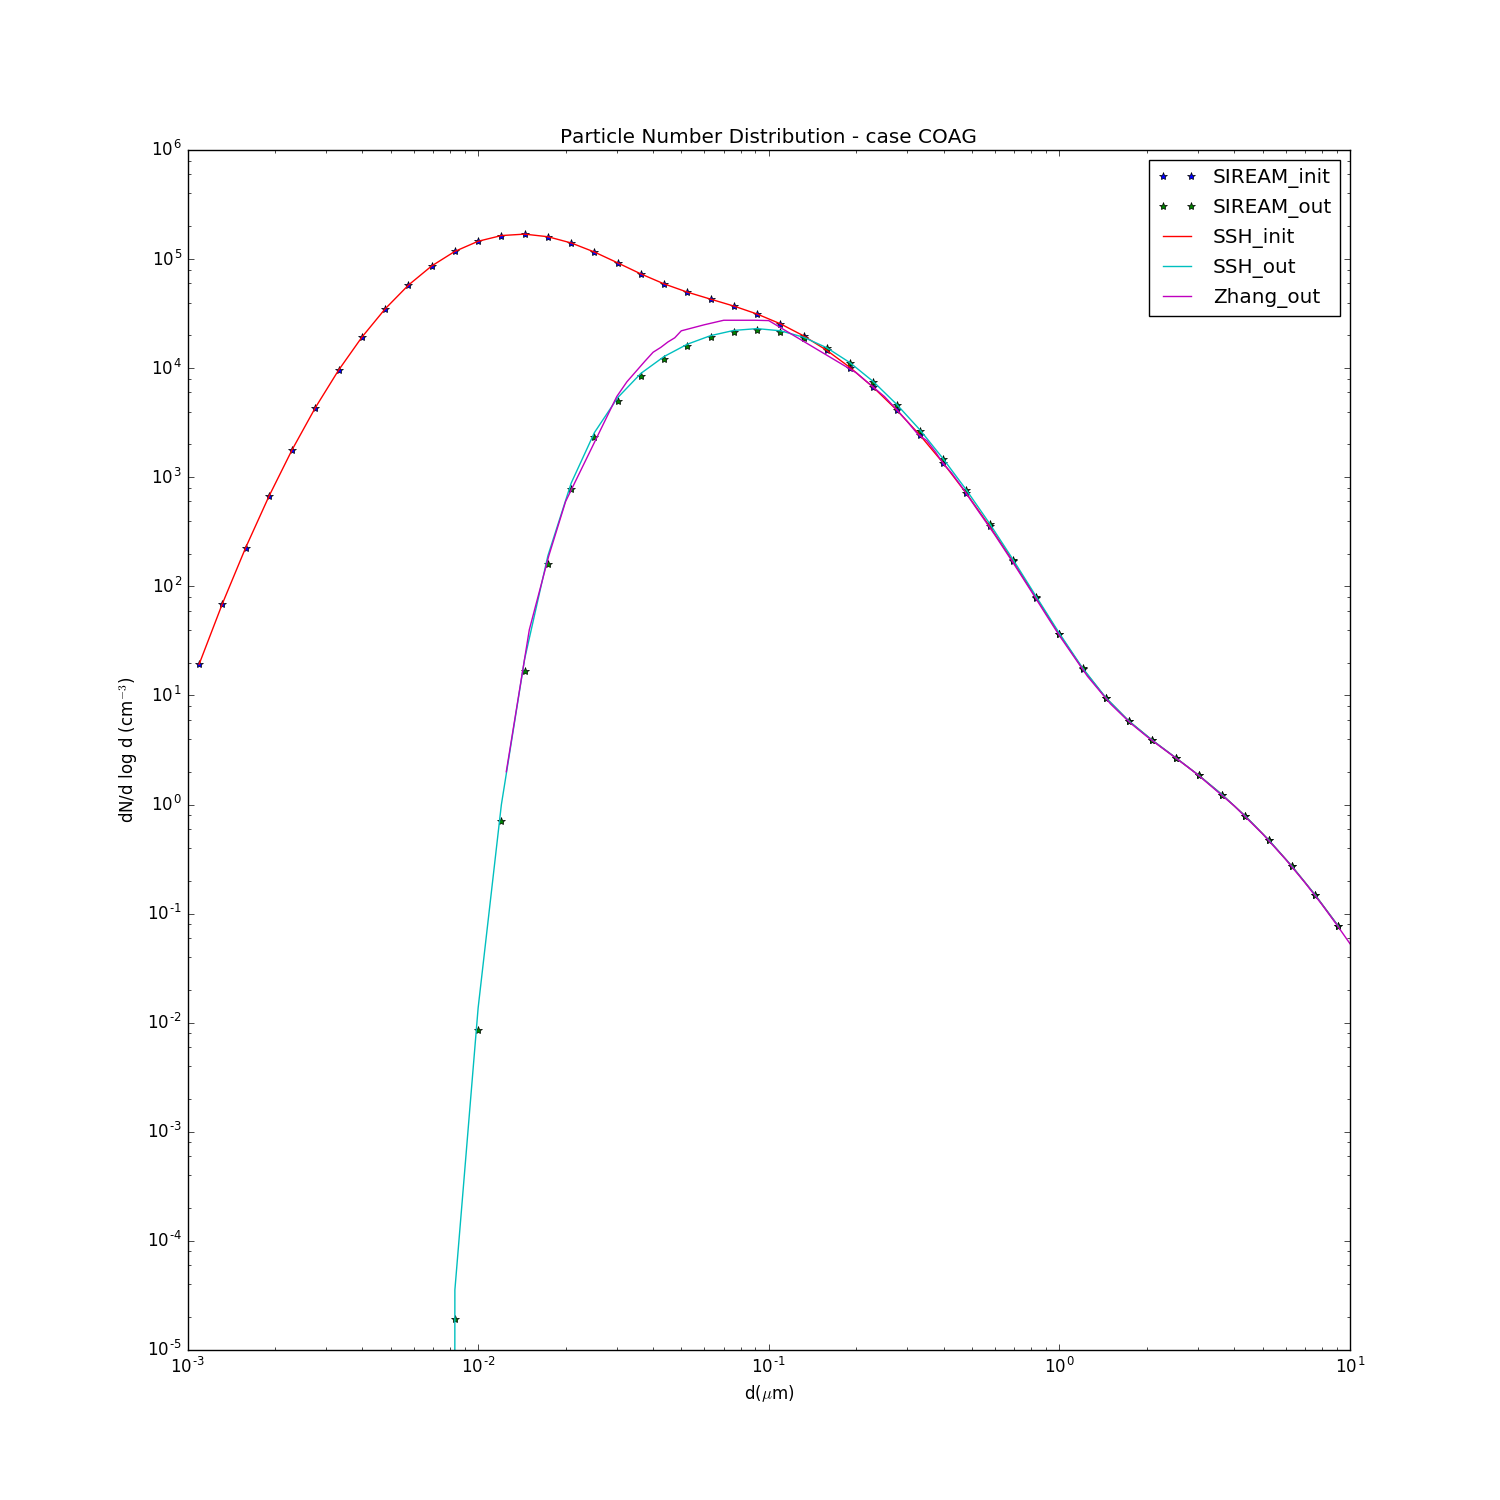
\includegraphics[angle=0,width=0.45\textwidth]{../graph/figure_ref/dNdlogd_COAG.png}
                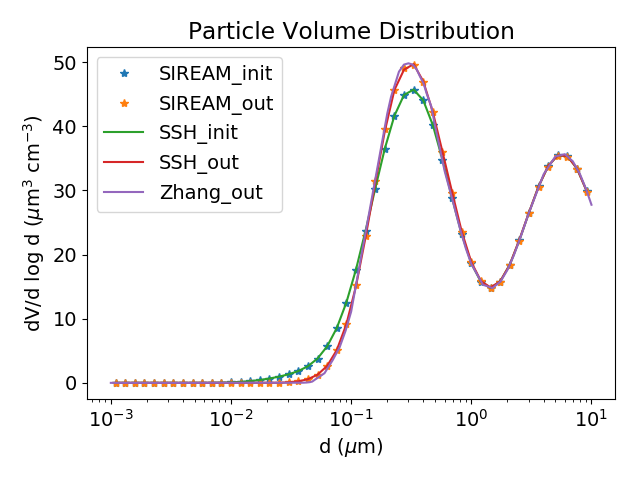
\includegraphics[angle=0,width=0.45\textwidth]{../graph/figure_ref/dVdlogd_COAG.png}
        \end{center}
\caption{Coagulation test case. Number (left panel) and volume (right panel) concentrations.}
\label{fig-coag}
\end{figure}
        
\subsubsection{Condensation of sulfate}
\label{cond-sulf}

The condensation test with hazy conditions is very stringent, because the high condensation
rate lead to a narrow Aitken mode.
The configuration file for this test is {\it{namelist\_cond.ssh}}.
Only condensation/evaporation is considered by setting the variable {\it{with\_cond}} of the file {\it{namelist.ssh}} to 1.

Run the simulation by typing {\it{ssh-aerosol INIT/namelist\_cond.ssh}}.
You can compare the number and volume distribution of particles at the initial
time and after 12~h by going to the repertory {\it{graph}} and by running the
python script {\it{dN\_Vdlogd\_cond.py}}.
SSH-aerosol does very well in representing
the Aitken mode as well as the growth of the accumulation mode if no
redistribution is used ({\it{redistribution\_method}} = 0 in
{\it{namelist\_cond.ssh}}), as shown in Fig~\ref{fig-cond-noredist}. 

Redistributing the mass and number concentrations
amongst bins lead to numerical diffusion, as can be seen by using the
redistribution methods 10 (moving diameter), 11 (area-based (siream)) or 12
(euler-coupled) (see Fig~\ref{fig-cond-redist}).
You can change the redistribution by changing the flag {\it{redistribution\_method}}.

In order to use a growth law, which is as close as possible to the original growth law
used in \cite{zhang1999simulation} , the accommodation coefficient is set to 1. It is however interesting
to notice the sensitivity of results to the choice of the accommodation coefficient. 
The growth of the Aitken mode is strongly reduced by decreasing the
accommodation coefficient from 1 to 0.1.
You can change the accomodation coefficient in the file {\it{species-list/species-list-aer.dat}}.

\begin{figure}[H]
        \begin{center}
                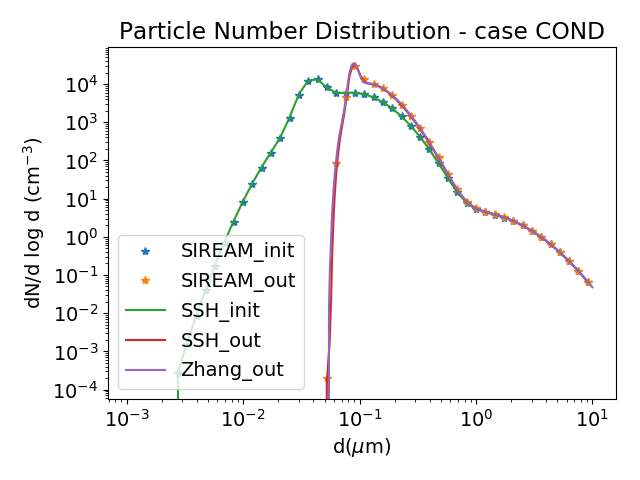
\includegraphics[angle=0,width=0.45\textwidth]{../graph/figure_ref/dNdlogd_COND_no_redist.png}
                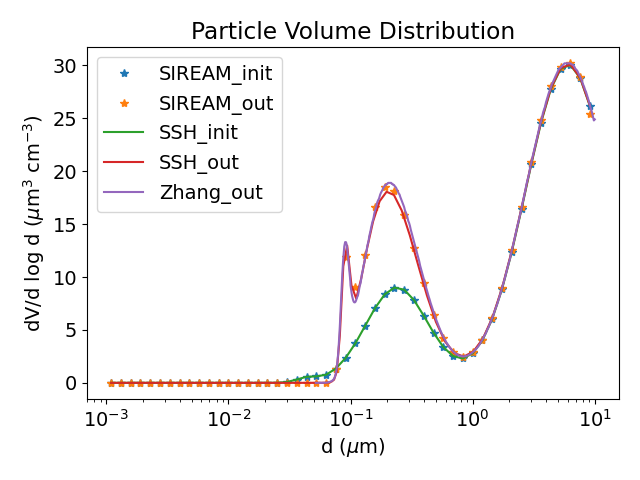
\includegraphics[angle=0,width=0.45\textwidth]{../graph/figure_ref/dVdlogd_COND_no_redist.png}
        \end{center}
\caption{Condensation test case without redistribution. Number (left panel) and volume (right panel) concentrations.}
\label{fig-cond-noredist}
\end{figure}
       
\begin{figure}[H]
        \begin{center}
                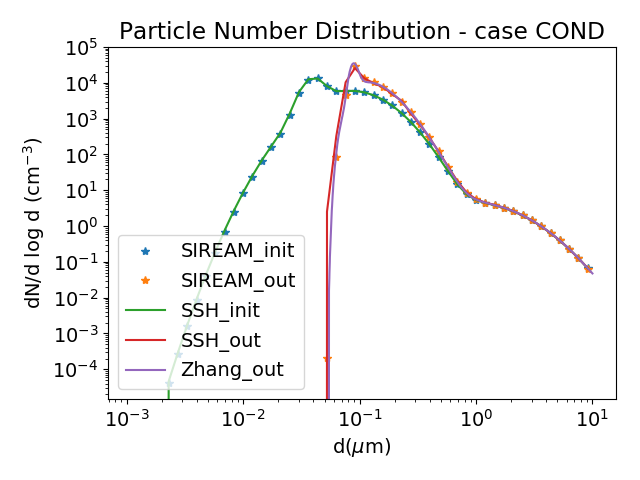
\includegraphics[angle=0,width=0.45\textwidth]{../graph/figure_ref/dNdlogd_COND_r12.png}
                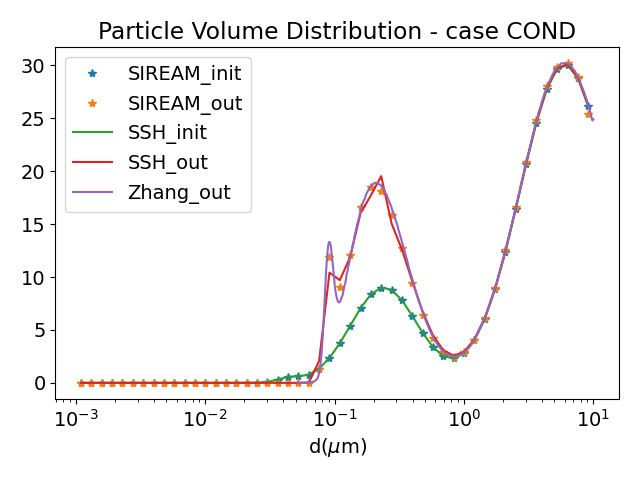
\includegraphics[angle=0,width=0.45\textwidth]{../graph/figure_ref/dVdlogd_COND_r12.png}
        \end{center}
\caption{Condensation test case with Euler-coupled redistribution. Number (left panel) and volume (right panel) concentrations.}
\label{fig-cond-redist}
\end{figure}
       
\subsubsection{Condensation of low-volatility organics}

Extremely-low volatility organic compounds (ELVOCs) are formed from the ozonolysis of monoterpenes \cite{chrit2017} .
Similarly to sulfate, these compounds have a very low saturation vapour pressure and they therefore should condense with a kinetic similar to sulfate if they had the same density.
The test case on the sulfate condensation is redone with the ELVOC Monomer, by artificially setting its density to that of sulfate.
The configuration file for this test is {\it{namelist\_cond\_monomer.ssh}}.
The monomer density is modified in the file {\it{species-list/species-list-aer-test.dat}}.
In the input files for initial conditions {\it{init\_gas.dat}} and {\it{init\_aero.dat}} of the directory {\it{inputs/inputs-cond-monomer/}}, initial concentrations are assigned to monomer rather than sulfate. You can plot the number and volume distribution by using the python script {\it{graph/dN\_Vdlogd\_cond\_monomer.py}}. 
The distributions are similar to those of the sulfate case.

\subsubsection{Condensation/evaporation of inorganics}
For inorganic compounds, differences between the particle compositions computed using equilibrium and dynamical sectional models have been stressed by numerous authors such as \cite{sartelet2006}. This test case simulates the test case of the highly polluted day of 25 June 2001 of \cite{sartelet2006} .
Measurements of PM and gaseous species made in Tokyo (Japan) are taken as initial conditions. Because the data were averaged continuously during 24 hours under varying meteorological conditions, this study can not assess the importance of the equilibrium approach compared to the dynamical approach. The model results obtained after thermodynamic equilibrium is reached are then compared.

The configuration file for this test is {\it{namelist\_cond-evap-inorg.ssh}} for the case where condensation/evaporation is dynamic. 
Only condensation/evaporation is considered by setting the variable of {\it{namelist\_cond-evap-inorg.ssh}} {\it{with\_cond}} to 1.
The variable {\it{Cut\_dim}} corresponds to the diameter until which thermodynamic is assumed. It is set to 0 to solve the condensation/evaporation with a dynamic approach. 

To compare this simulation to a simulation where thermodynamic equilibrium is assumed for condensation/evaporation, please set  {\it{Cut\_dim}} to 40 (the maximum diameter of the particles considered here). 
This is done in the configuration file {\it{namelist\_cond-evap-inorg-eq.ssh}}.

A hybrid method may also be used to compute condensation/evaporation: thermodynamic equilibrium is then computed only for size sections of mean diameter lower than a cutoff diameter, while condensation/evaporation is computed dynamically for size sections of diameter higher than the cutoff diameter. For example, a cutoff diameter {\it{Cut\_dim}} of 0.1~$\mu$m is set in the configuration file {\it{namelist\_cond-evap-inorg-icut.ssh}}.


To assess the differences between these simulations, you can compare the time evolution of NH$_3$ and HNO$_3$, 
by running the python script {\it{graph/gas\_cond-evap.py}}. As shown in
Fig~\ref{fig-cond-evap}, the gas-phase concentrations quickly reach
thermodynamic equilibrium. The concentrations computed with the hybrid approach are close to those computed by the dynamic approach.


\begin{figure}[H]
        \begin{center}
                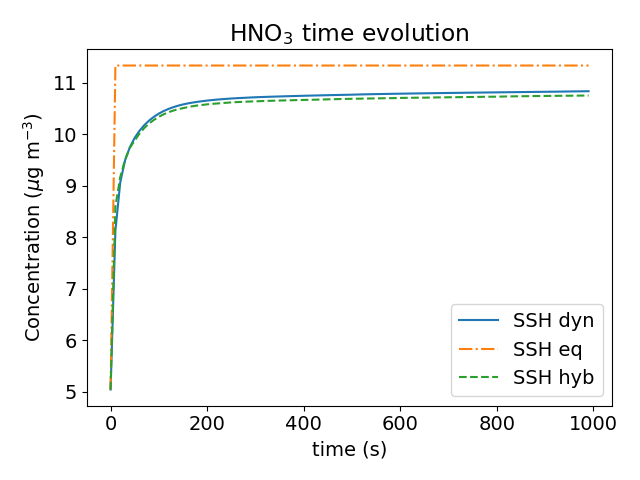
\includegraphics[angle=0,width=0.45\textwidth]{../graph/figure_ref/HNO3_COND-EVAP_time.png}
                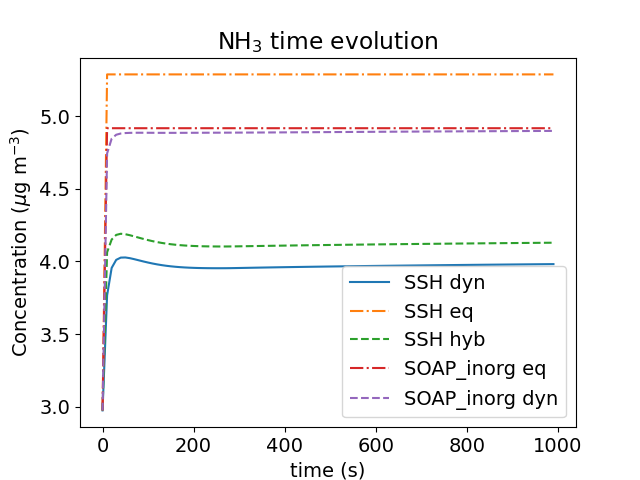
\includegraphics[angle=0,width=0.45\textwidth]{../graph/figure_ref/NH3_COND-EVAP_time.png}
        \end{center}
\caption{Condensation/\'evaporation of inorganic test case. Time evolution of
  HNO$_3$ concentrations (left panel) and NH$_3$ concentrations (right panel).}
\label{fig-cond-evap}
\end{figure}
       

\subsubsection{Kelvin effect}

To illustrate the importance of the Kelvin effect for the growth of ultrafine
particles, the test case of \cite{devilliers13} concerning the growth of
ultrafine particles emitted from the exhaust of a diesel engine was simulated.
As in \cite{devilliers13}, a typical diesel engine emission initial
distribution from \cite{kittelson2006road} is used here to
study the gas/particle conversion of nonadecane (C19H40). It has a
reference saturation vapour pressure of 6.1~10$^{-4}$ Pa at T = 298 K, which is
very close to that of the model compound POAmP.
Particles are assumed here to consist solely of POAmP.
To show the importance of the Kelvin effect, two simulations are conducted:
with and without the Kelvin effect.

The configuration files for this test are {\it{namelist\_kelvin.ssh}} for the
case where the Kelvin effect is modelled, and {\it{namelist\_kelvin\_nokelv.ssh}} for the
case where it is not.
The variable {\it{ISOAPDYN}} is set to 1 to indicate that the
condensation/evaporation of organics is modelled dynamically. The variable
{\it{with\_kelvin\_effect}} is also set to 1 to take into account the Kelvin
effect in the configuration file {\it{namelist\_kelvin.ssh}} and to 0 in the configuration file {\it{namelist\_kelvin\_nokelv.ssh}}.

To compare the number and volume size distribution simulated with and without
Kelvin effect, you can run the python script {\it{graph/dN\_Vdlogd\_kelvin.py}}.

The results in Fig~\ref{fig-kelvin} show clearly that the Kelvin effect must be taken into account when
the evolution of small particles is simulated: particles are much less affected by
condensation/evaporation when it is not included in the model. The ultrafine particles of the initial distribution have been transferred to the gas phase while the coarse ones have grown to a greater size range.



\begin{figure}[H]
        \begin{center}
                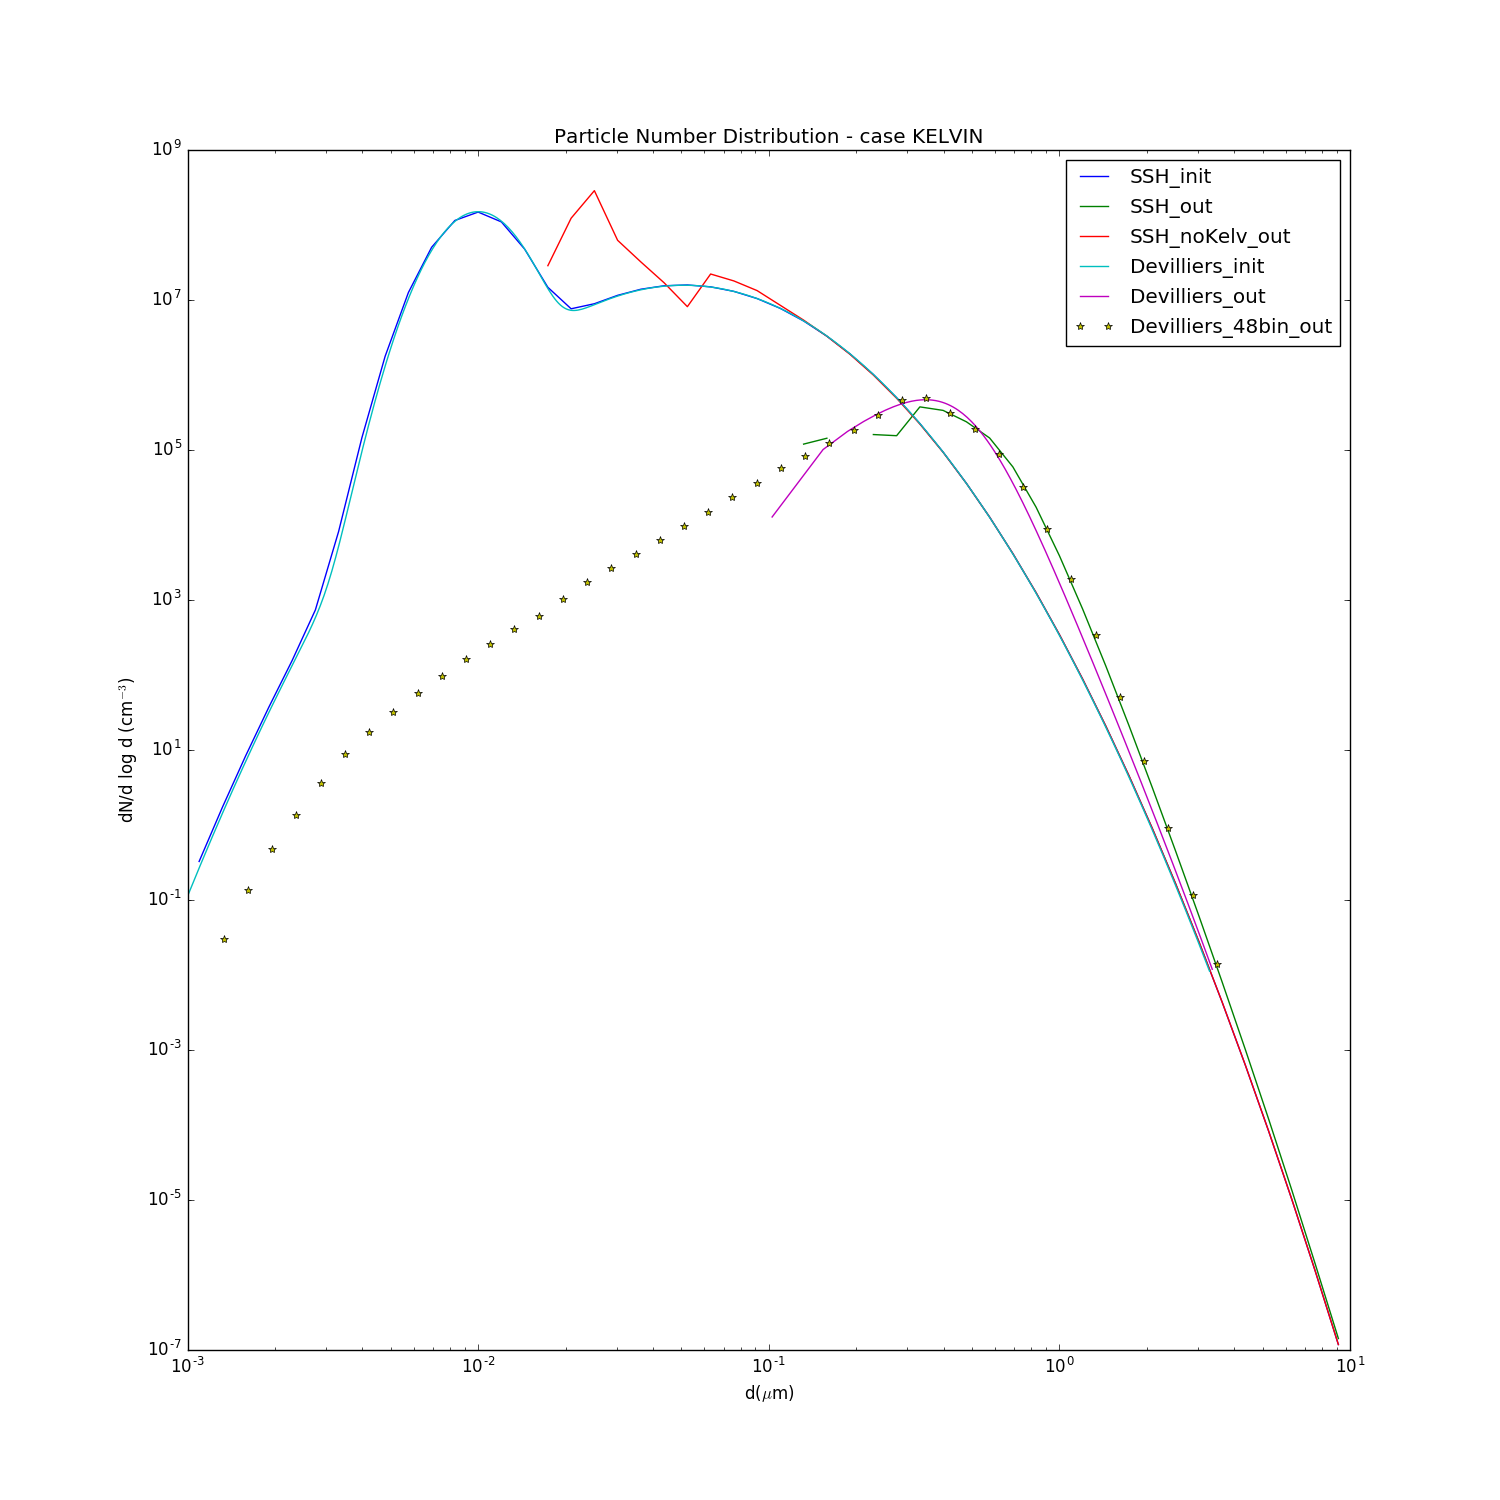
\includegraphics[angle=0,width=0.45\textwidth]{../graph/figure_ref/dNdlogd_KELVIN.png}
                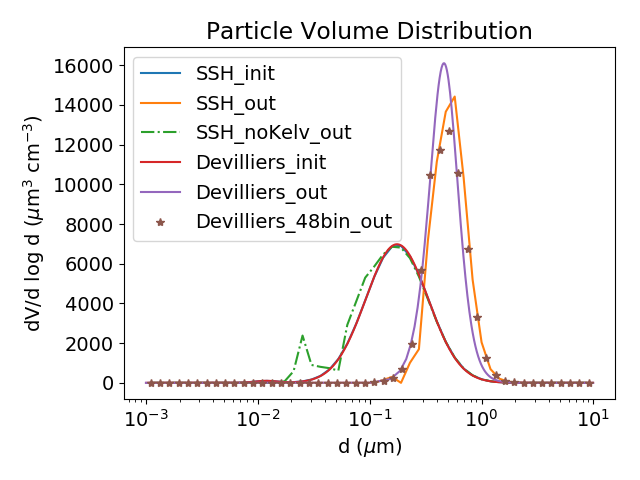
\includegraphics[angle=0,width=0.45\textwidth]{../graph/figure_ref/dVdlogd_KELVIN.png}
        \end{center}
\caption{Kelvin test case. Number (left panel) and volume (right panel) concentrations.}
\label{fig-kelvin}
\end{figure}
       
\subsubsection{Nucleation}

To assess the ability of SSH-aerosol to deal with simultaneous strong coagulation and condensation/nucleation, the nucleation test case presented in \cite{sartelet2006} is simulated. The initial distribution is the same as in the condensation of sulphuric acid test case of section~\ref{cond-sulf}. It corresponds to the hazy conditions of \cite{seigneur1986simulation}. The sulphuric
acid production rate is 0.825~$\mu$g~m$^{-3}$~h$^{-1}$,
the temperature is 288.15 K and the relative humidity is 60\%. The particles are initially assumed to be made of 70\% sulfate and 30\% ammonium. The initial gas phase ammonia concentration is taken to be 8~$\mu$g~m$^{-3}$. The concentrations of gas phase ammonia and particulate-phase ammonium evolve with time due to both nucleation and condensation/evaporation
The ternary nucleation of \cite{napari} is used, but to avoid artificially large nucleation rates in the parameterisation of \cite{napari}, a maximum nucleation rate of 1.d6 \#particles~cm$^{-3}$ is set.
The simulation is run for 1~h with output every 60~s.

Two simulations are run: one where the processes (coagulation,
condensation/evaporation and nucleation) are solved simultaneously
(configuration file {\it{namelist\_nucl.ssh}}), and one where the numerical
resolution of coagulation is splitted from condensation/evaporation and
nucleation (configuration file {\it{namelist\_nucl\_split.ssh}}). 

To compare the number and volume size distribution simulated with the two numerical algorithms, you can run the python script {\it{graph/dN\_Vdlogd\_nucl.py}}.

The two numerical algorithms give similar number concentrations, as shown in Fig~\ref{fig-nucl}.

The nucleated particles clearly grow to larger particles with time, as can be seen both in Fig~\ref{fig-nucl2} and by running the python script {\it{graph/banana.py}}.

Ultra-fine particles grow under the combined effect of coagulation,
condensation of sulphate and nucleation. 
As shown in Figure~\ref{fig-nucl2}, the nucleated particles clearly grow to larger particles with time.
This growth can be accelerated by the presence low-volatility compounds, as shown in \cite{pat18}, underlying the importance of an accurate modelling of the formation of ELVOCs for the growth of ultra-fine particles. 
The simulation of Figures~\ref{fig-nucl} and~\ref{fig-nucl2} is redone by adding 1~$\mu$g~m$^{-3}$ of a SSH-aerosol surrogate, Monomer, which is an ELVOC formed from the oxidation of terpenes (configuration file {\it{namelist\_nucl\_org.ssh}}).
To compare the number and volume size distribution simulated with/without the surrogate Monomer, you can run the python script {\it{graph/dN\_Vdlogd\_nucl\_org.py}}.
As shown in Figure~\ref{fig-nucl3}, the comparison of the number concentration simulated with and without taking the surrogate Monomer into account shows that 
the particles have grown to larger diameters because of the presence of Monomer. 
The left panel of Figure~\ref{fig-nucl2} shows the time evolution of the number concentration for the different size sections without Monomer (script {\it{graph/banana.py}}) and 
the right panel of Figure~\ref{fig-nucl2} shows the same time evolution but with 1~$\mu$g~m$^{-3}$ of the surrogate Monomer condensing (script {\it{graph/banana\_org.py}}). 
The surrogate Monomer first condenses to existing particles around 0.01~$\mu$m, making them grow to larger diameters.
Note that the condensation of the extremely low-volatility surrogate Monomer needs to be solved simultaneously to coagulation and nucleation to correctly represent this growth of ultra-fine particles (the parameter non\_volatile needs to be set to 1 for the surrogate Monomer in the input file {\it{species-list/species-list-aer.dat}}).

\begin{figure}[H]
        \begin{center}
                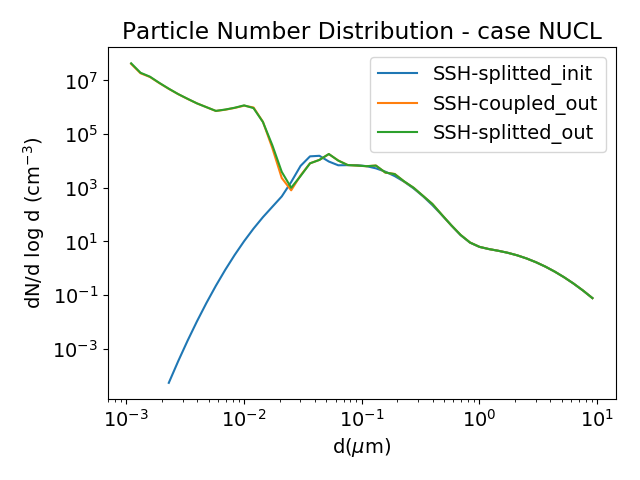
\includegraphics[angle=0,width=0.45\textwidth]{../graph/figure_ref/dNdlogd_nucl.png}
                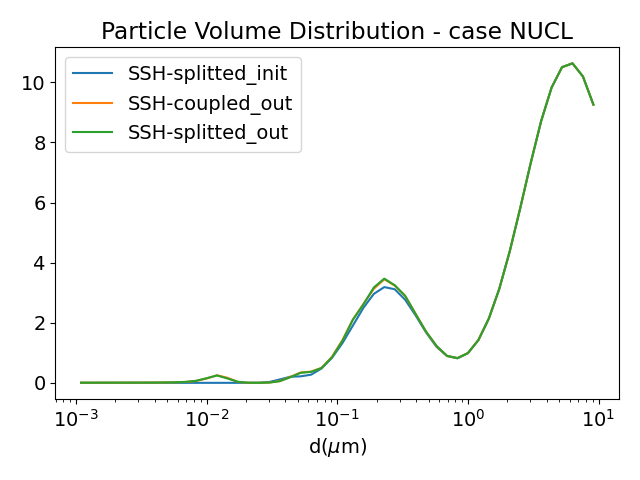
\includegraphics[angle=0,width=0.45\textwidth]{../graph/figure_ref/dVdlogd_nucl.png}
        \end{center}
\caption{Nucleation test case. Number (left panel) and volume (right panel) concentrations.}
\label{fig-nucl}
\end{figure}

\begin{figure}[H]
        \begin{center}
                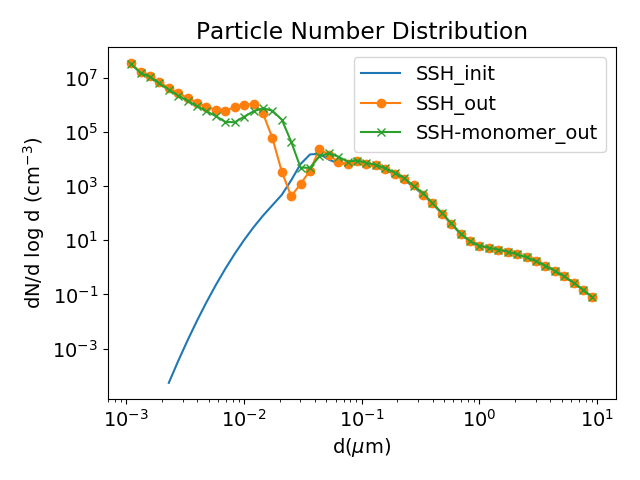
\includegraphics[angle=0,width=0.45\textwidth]{../graph/figure_ref/dNdlogd_nucl_org.png}
                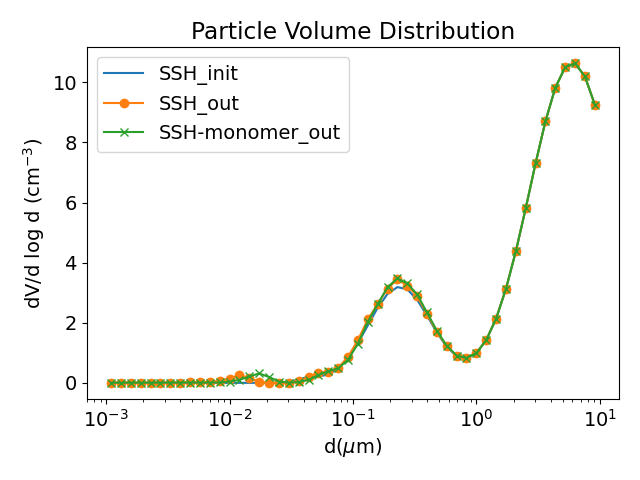
\includegraphics[angle=0,width=0.45\textwidth]{../graph/figure_ref/dVdlogd_nucl_org.png}
        \end{center}
\caption{Nucleation test case with Monomer surrogate added. Number (left panel) and volume (right panel) concentrations.}
\label{fig-nucl3}
\end{figure}
       
       

\begin{figure}[H]
        \begin{center}
                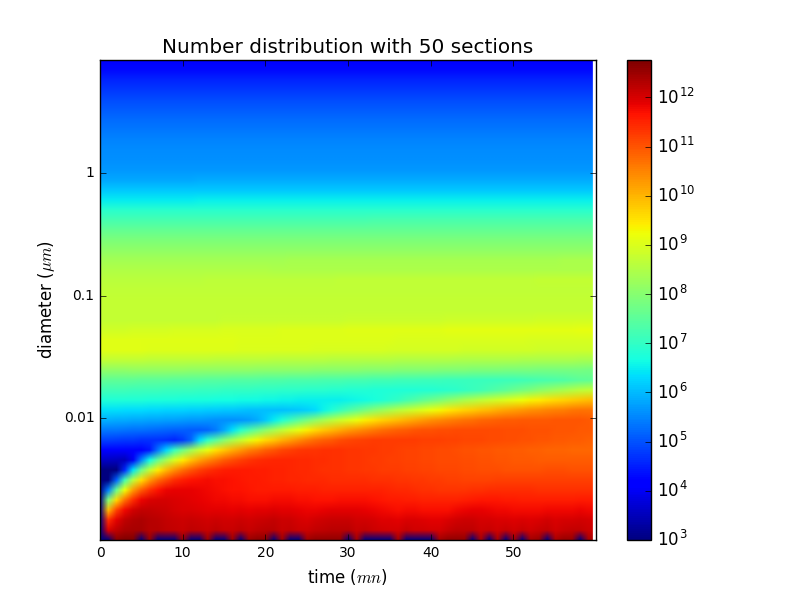
\includegraphics[angle=0,width=0.45\textwidth]{../graph/figure_ref/fig_banana.png}
                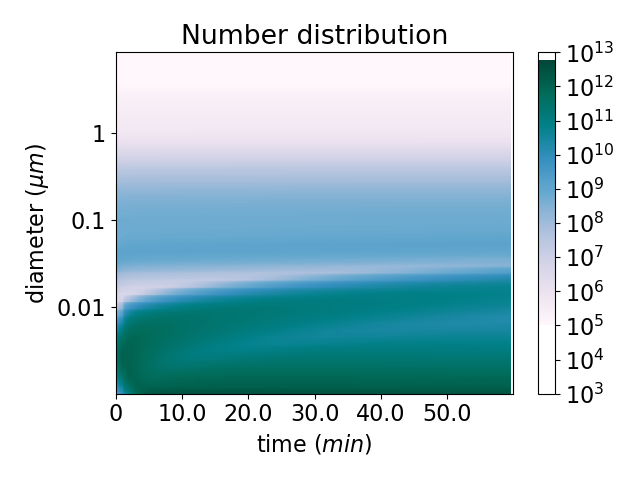
\includegraphics[angle=0,width=0.45\textwidth]{../graph/figure_ref/fig_banana_org.png}
        \end{center}
\caption{Nucleation test case. Time evolution of the number concentrations. Without organics (right panel), with organics (surrogate Monomer, left panel).}
\label{fig-nucl2}
\end{figure}
       

\subsection{Modelling of aerosol formation}

After emission into the atmosphere, the oxidation of volatile organic compounds (VOCs) leads to less volatile compounds than the precursors. 
These compounds condense more easily onto particles than their precursors and they contribute to the increase of particle mass.

\subsubsection{Formation of condensable}

\cite{platt2013secondary} performed ageing experiments on emissions from an Euro 5 gasoline car. They monitored the total hydrocarbon mass (THC) as well as organic aerosol (OA) concentrations. 
The test case presented here corresponds to the simulation performed in \cite{sartelet2018}.

In our model, THC is assumed to be the sum of VOC and I/S VOCs (intermediate and semi-volatile VOCs). THC is initialised as measured in the experiments of \cite{platt2013secondary} before lights-on (1.4 ppmv + 0.9 ppmv of propene). IVOCs are estimated from VOC emissions using the ratio 0.17 estimated by \cite{zhao2016intermediate}, and NOx concentrations are initialised such as having a VOC/NOx ratio equal to 5.6 as in \cite{platt2013secondary} . 
The speciation of VOCs to model species was done following \cite{theloke2007}.

The configuration file for this test is {\it{namelist\_platt.ssh}}.

Not only condensation/evaporation is considered by setting the variable of {\it{namelist\_platt.ssh}} {\it{with\_cond}} to 1, but also gaseous chemistry ( {\it{tag\_chem}}=1). Predefined photolysis rates may be used, or tabulated values may be downloaded.

After running the model for 5~h, the evolution of the aerosol concentrations with time may be displayed by running the script {\it{plot\_platt\_particles.py}}.
As in the experiment after correction for wall loss, the concentrations of
particles is about 200~$\mu g$~$m^{-3}$. More than half of the mass origins
from the condensation/evaporation of aged I/S VOCs, as shown in Fig~\ref{fig-platt}.
The inorganic concentrations stay very low, as only 0.1~$\mu g$~$m^{-3}$) of sulfate and ammonium were introduced.

Ammoniac emission was not considered in the previous test case. However, to reduce NOx emissions, ammoniac may also be emitted by recent vehicles \cite{suarez17}. 
To illustrate the potential influence of NH$_3$ emission on secondary aerosol formation, the initial conditions of the test case above are modified to include NH$_3$ emissions, assumed to be 10\% of NOx emissions \cite{suarez17}. 
The configuration file for this test is {\it{namelist\_platt\_nh3.ssh}}.
After running the model, the evolution of the aerosol concentrations with time may be displayed by running the script {\it{plot\_platt\_particles\_nh3.py}}.
As shown in Figure~\ref{fig-platt}, NH$_3$ emission leads to a large increase in inorganic aerosol concentrations (from 0.1~$\mu$g~m$^{-3}$ to about 37~$\mu$g~m$^{-3}$).

\begin{figure}[H]
        \begin{center}
                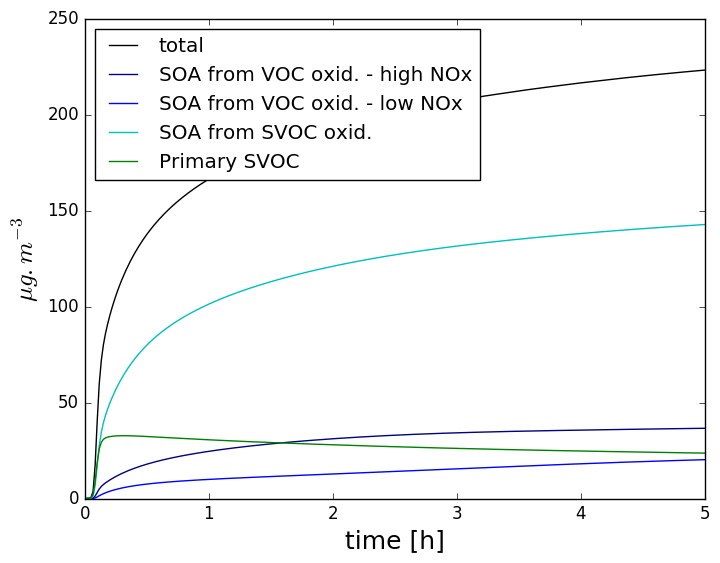
\includegraphics[angle=0,width=0.45\textwidth]{../graph/figure_ref/platt-particles.png}
                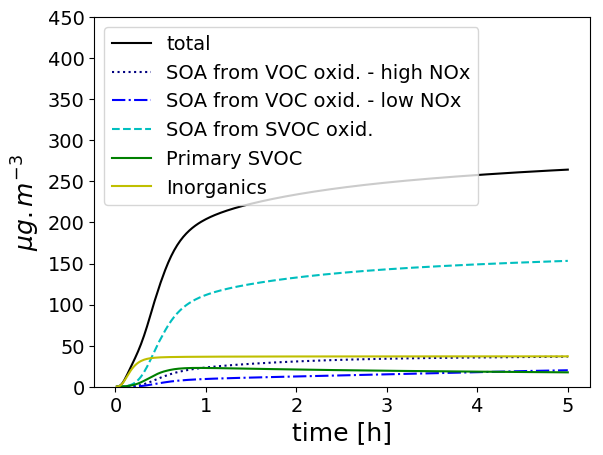
\includegraphics[angle=0,width=0.45\textwidth]{../graph/figure_ref/platt-particles-nh3.png}
        \end{center}
	\caption{Time evolution of organic and inorganic concentrations for the Platt test case: without NH$_3$ emissions (left panel), with NH$_3$ emissions (right panel).}
\label{fig-platt}
\end{figure}

\subsubsection{Absorption into an aqueous or an organic phase}
\label{hybhyd}

The SOA compounds formed from the exhaust are assumed to be mostly hydrophobic, and
therefore condense onto an organic phase. SOA compounds formed from biogenic precursors have a stronger affinity with water \cite{couvidat11, couvidat2012}, and they may prefer condensing onto an aqueous phase, formed by hydrophilic organic compounds and water absorbed by inorganics and hydrophilic organic compounds \cite{kim2019}.
To illustrate the influence of hygroscopicity, the exhaust test case of the previous section is simulated by adding 150~$\mu$g~m$^{-3}$ of isoprene. In the case when NH$_3$ is not emitted in the exhaust, biogenic condensables are formed but mostly stay in the gas phase, because they are mostly hydrophilic and 
they can not condense efficiently on the hydrophobic particles formed from the exhaust emission.
As shown in Figure~\ref{fig-platt-isop}, if NH$_3$ is added to the exhaust, inorganic aerosol concentrations largely increase, leading to an increase in isoprene SOA, which can then condense onto aqueous particles.

In the previous test case, the influence of activity coefficients on the SOA formation is not taken into account. 
Depending on the user's choice, short-range or short, medium and long-range activity coefficients can be modelled. If only short-range activity coefficients (interactions between uncharged molecules) are modelled, then they are computed using the UNIQUAC Functional-group Activity Coefficients (UNIFAC) thermodynamic model \cite{Fredenslund}, 
which is based on a functional group method. If short, medium and long-range activity coefficients are modelled, i.e. taking into account the influence of inorganic ions in the SOA aqueous phase, they are computed using the Aerosol Inorganic-Organic Mixtures Functional groups Activity Coefficients (AIOMFAC) model \cite{zuend2008}. 

The configuration file for the test case of exaust emissions with added isoprene emission is {\it{namelist\_platt\_nh3\_isop.ssh}}.
Two other simulations may also be run using UNIFAC to compute activity coefficients ({\it{namelist\_platt\_nh3\_isopu.ssh}}) or AIOMFAC ({\it{namelist\_platt\_nh3\_isopa.ssh}}).

The evolutions of the concentrations of isoprene SOA in particles as a function of time for these simulations may be seen in Figure~\ref{fig-platt-isop}, which can be plotted runing the script {\it{platt\_isop.py}}.
As already shown in the 3D studies of \cite{couvidat2012, kim2019}, and as shown here in Figure~\ref{fig-platt-isop} for isoprene SOA, ideality strongly influences the partitioning between the gas and particle phase. 
\begin{figure}[H]
        \begin{center}
                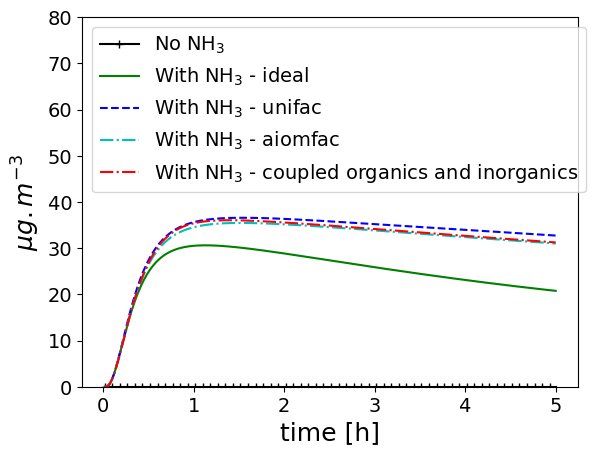
\includegraphics[angle=0,width=0.45\textwidth]{../graph/figure_ref/platt-isop.png}
        \end{center}
	\caption{Time evolution of isoprene SOA in the particle phase.}
\label{fig-platt-isop}
\end{figure}
      

\subsection{Mixing state}
The previous test cases relied on the internal mixing assumption (one aerosol
composition per aerosol size section).
The internal mixing assumption relies on the assumption that particles from different sources
mix instantaneously when they are present in the same air mass. Although this assumption may
be realistic far from emission sources, it may be difficult to justify close to emission sources,
where emitted particles can have compositions that are very different from background particles
and from particles emitted from different sources.
All aerosol dynamic processes may affect the mixing state of particles.

\subsubsection{Coagulation}

To illustrate how coagulation affects the mixing state of particles, the
coagulation test case (see section~\ref{coag-test}) is revisited by assuming
that the initial aerosol distribution is made of two low-volatility compounds
of same density (sulfate and another low-volatility compound).
The configuration file for this test is {\it{namelist\_coag\_ext.ssh}}.
In this coagulation test case, the composition is discretized using 4 sections
by setting the variable {\it{N\_frac}} to 4. The bound values of the fraction
sections are specified using the variable {\it{frac\_input}}.

Run the simulation by typing {\it{ssh-aerosol INIT/namelist\_coag\_ext.ssh}}.
By summing the mass and number of particles of all size fraction sections, the
size number and volume distribution are identical to those obtained with the
internal mixing assumptions. This can be checked by going to the repertory
{\it{graph}} and by running the python script {\it{dN\_Vdlogd\_coag\_ext.py}}
(see Fig~\ref{fig-coag-ext}).
The python script {\it{coag\_2D.py}} allows to create figures to visualize the initial and final mass concentrations as a function of size and fraction of sulfate.
Hence, the evolution of the mixing-state of particles after 12 h of coagulation may
be seen by comparing the two panels in Fig~\ref{fig-coag-extb}, which shows
the number concentrations as a function of the size and fraction of 
sulfate, which is one of the
two compounds of the particles.

\begin{figure}[H]
        \begin{center}
                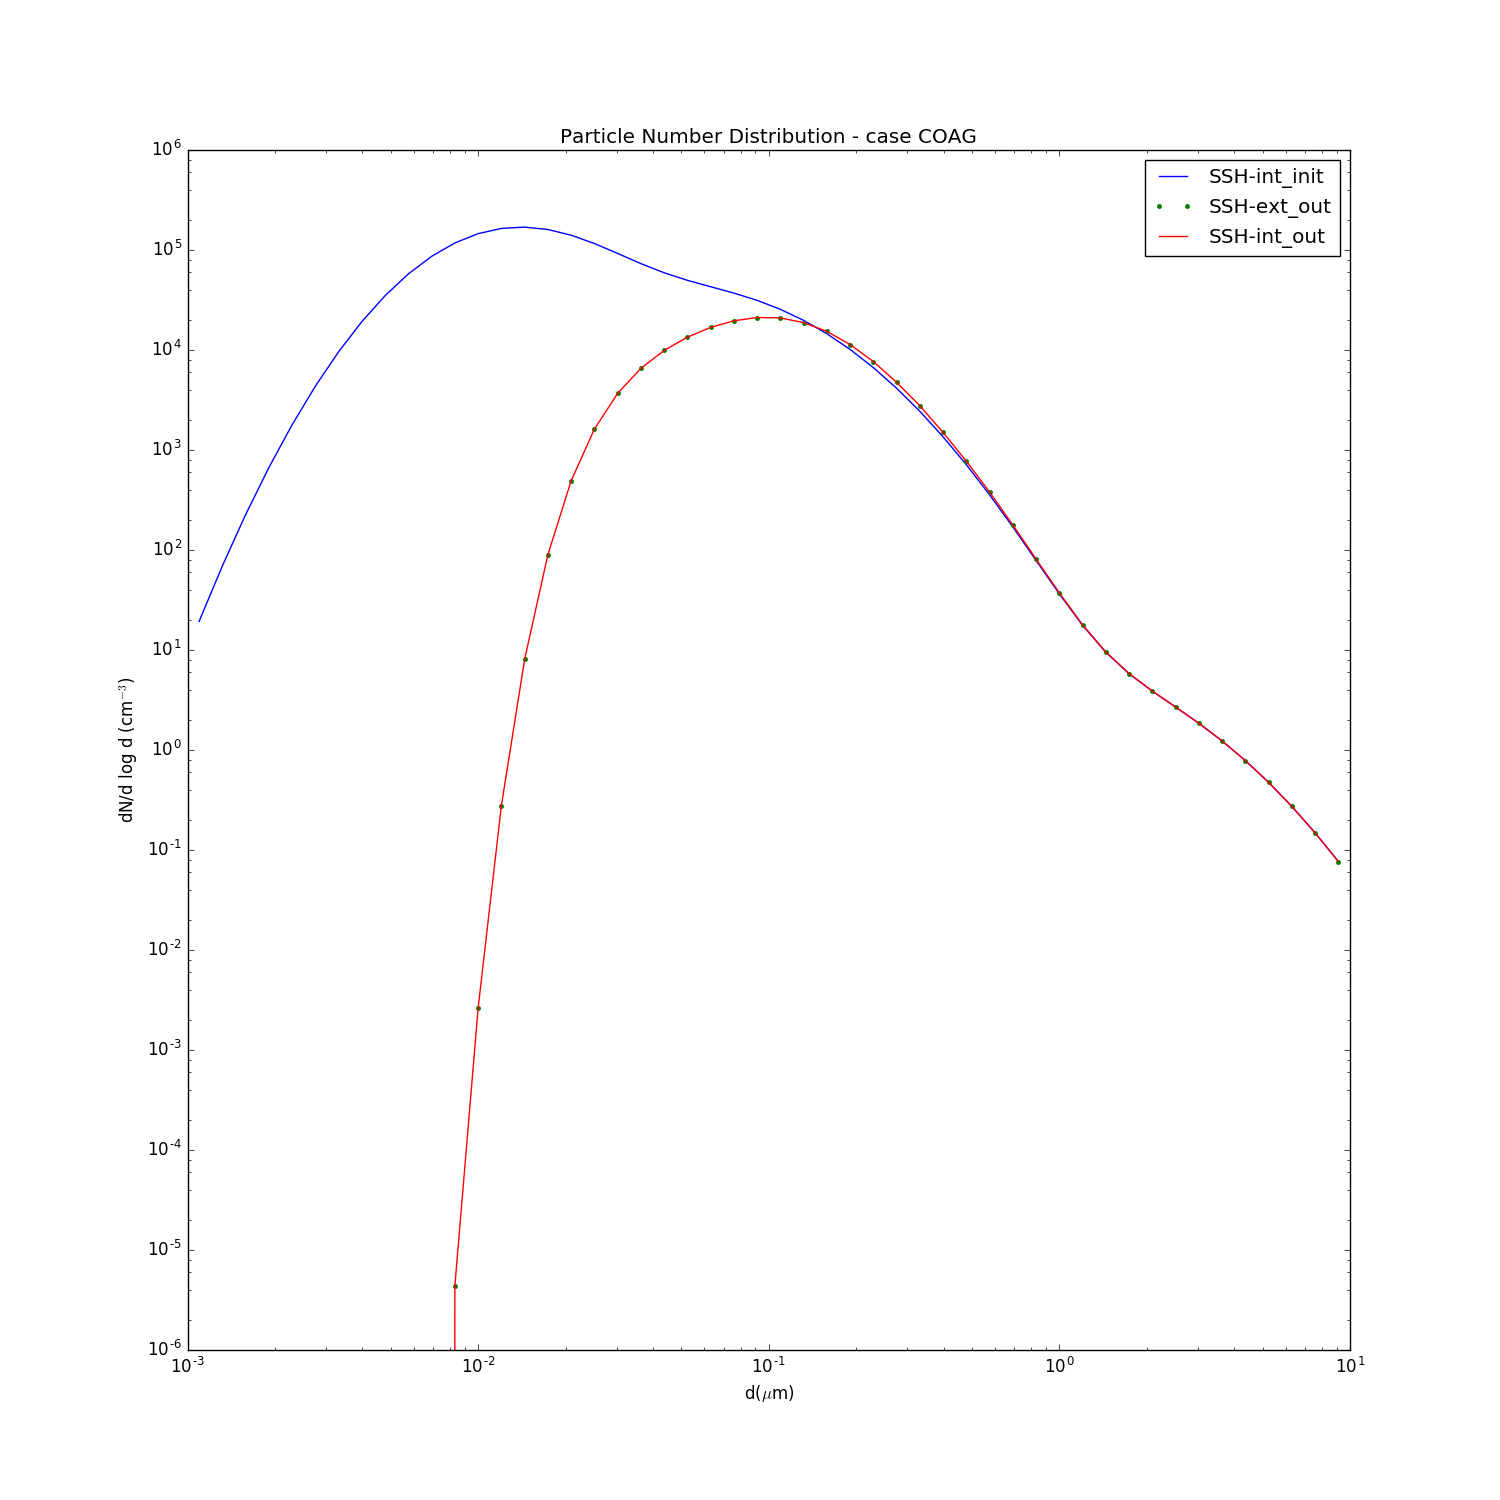
\includegraphics[angle=0,width=0.45\textwidth]{../graph/figure_ref/dNdlogd_COAG_EXT.png}
                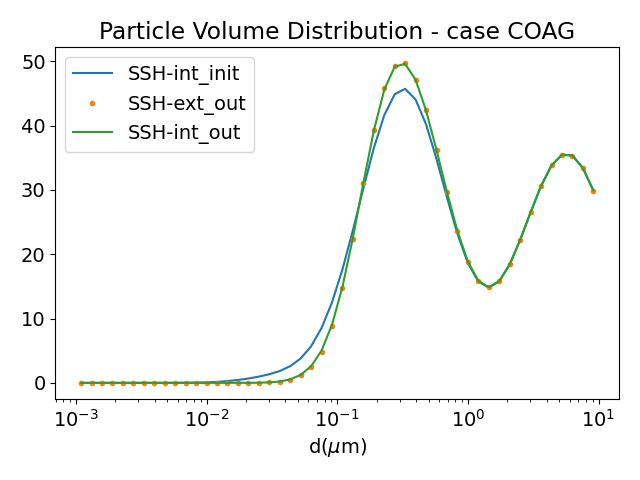
\includegraphics[angle=0,width=0.45\textwidth]{../graph/figure_ref/dVdlogd_COAG_EXT.png}
        \end{center}
\caption{Coagulation test case with mixing-state modelling. Number (left panel) and volume (right panel) concentrations.}
\label{fig-coag-ext}
\end{figure}
 
\begin{figure}[H]
        \begin{center}
                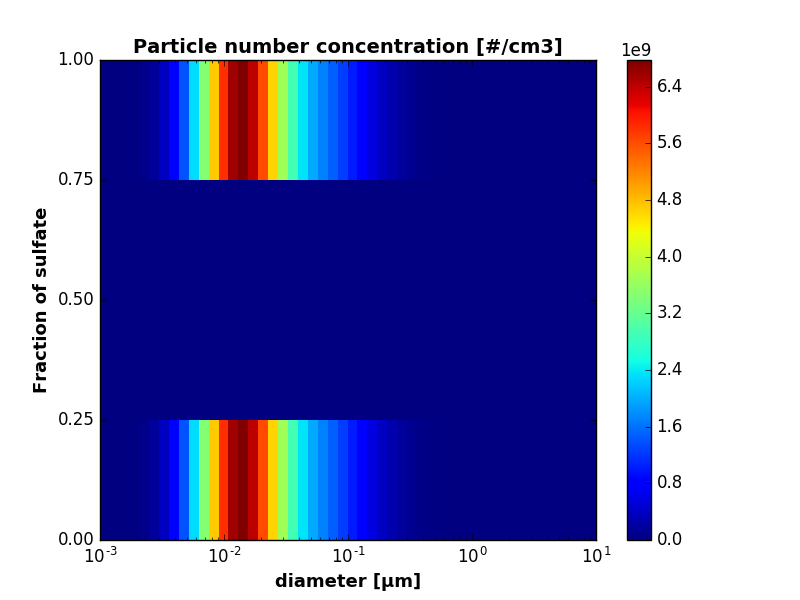
\includegraphics[angle=0,width=0.45\textwidth]{../graph/figure_ref/coag_ext_init.png}
                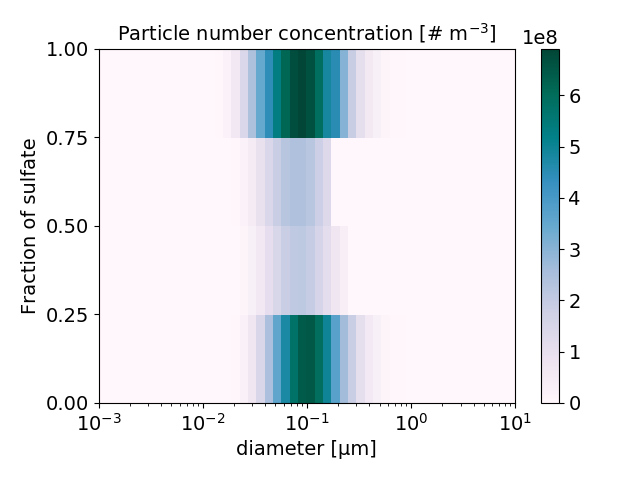
\includegraphics[angle=0,width=0.45\textwidth]{../graph/figure_ref/coag_ext_out.png}
        \end{center}
\caption{Number concentrations as a function of the size and fraction of one of the
two compounds at initial time (left panel) and after 12 h of simulation (right panel).}
\label{fig-coag-extb}
\end{figure}
 
\subsubsection{Condensation}

The effect of 
condensation on the mixing state is assessed by revisiting the condensation
test case (typical of a regional haze scenario, see section~\ref{cond-sulf}) by assuming
that the initial aerosol distribution is made of two low-volatility compounds
of same density (sulfate and another low-volatility compound).
As in \cite{zhu2015}, 10 composition fractions are used.
The configuration file for this test is {\it{namelist\_cond\_ext.ssh}}.
Run the simulation by typing {\it{ssh-aerosol INIT/namelist\_cond\_ext.ssh}}.
By summing the mass and number of particles of all size fraction sections, the
size number and volume distribution are identical to those obtained with the
internal mixing assumptions. This can be checked by going to the repertory
{\it{graph}} and by running the python script {\it{dN\_Vdlogd\_cond\_ext.py}}
(see Fig~\ref{fig-cond-ext}).
The python script {\it{cond\_2D.py}} allows to create figures to visualize the initial and final mass concentrations as a function of size and fraction of sulfate.
Hence, the evolution of the mixing-state of particles after 12 h of condensation and coagulation may
be seen by comparing the two panels in Fig~\ref{fig-cond-extb}, which shows
the mass concentrations as a function of the size and fraction of
sulfate, which is one of the
two compounds of the particles. 
Sulphuric acid condenses to form
sulfate. Because the condensation rate is greater for particles of
low diameters, the sulfate fraction is greater for those particles at the end
of the simulation (Figure~\ref{fig-cond-extb}).


\begin{figure}[H]
        \begin{center}
                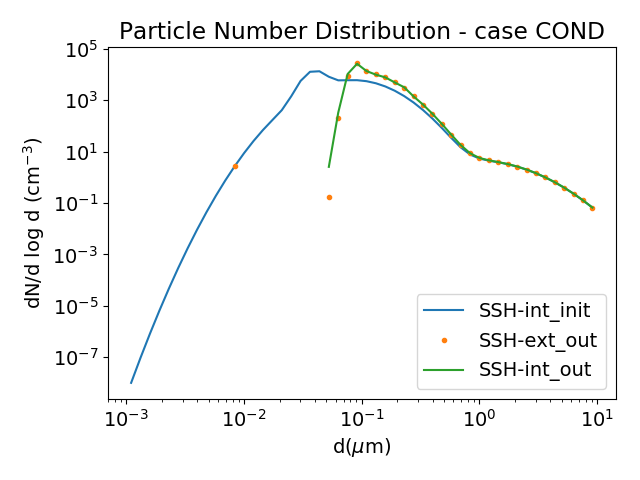
\includegraphics[angle=0,width=0.45\textwidth]{../graph/figure_ref/dNdlogd_COND_EXT.png}
                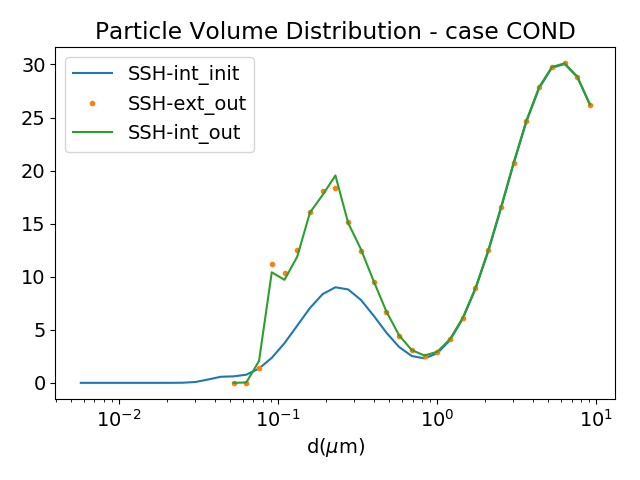
\includegraphics[angle=0,width=0.45\textwidth]{../graph/figure_ref/dVdlogd_COND_EXT.png}
        \end{center}
\caption{Regional haze test case with mixing-state modelling. Number (left panel) and volume (right panel) concentrations.}
\label{fig-cond-ext}
\end{figure}
 
\begin{figure}[H]
        \begin{center}
                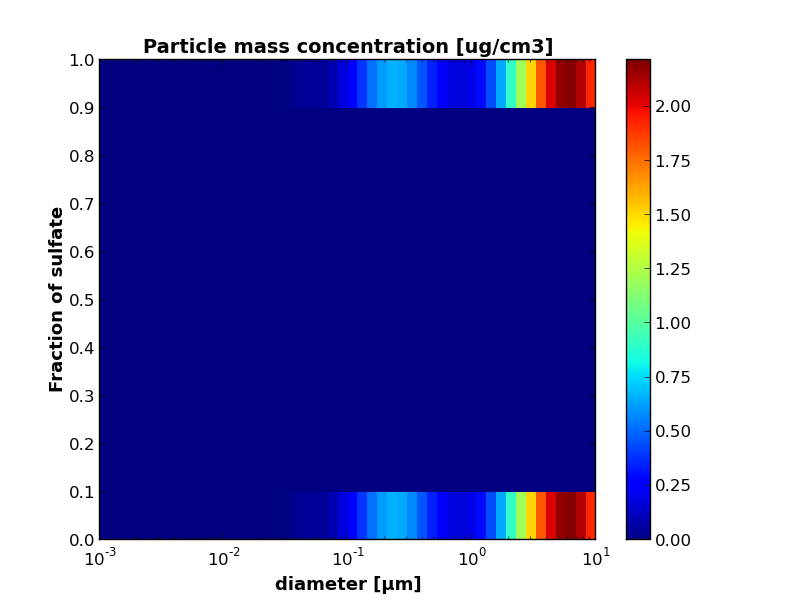
\includegraphics[angle=0,width=0.45\textwidth]{../graph/figure_ref/cond_mass_ext_init.png}
                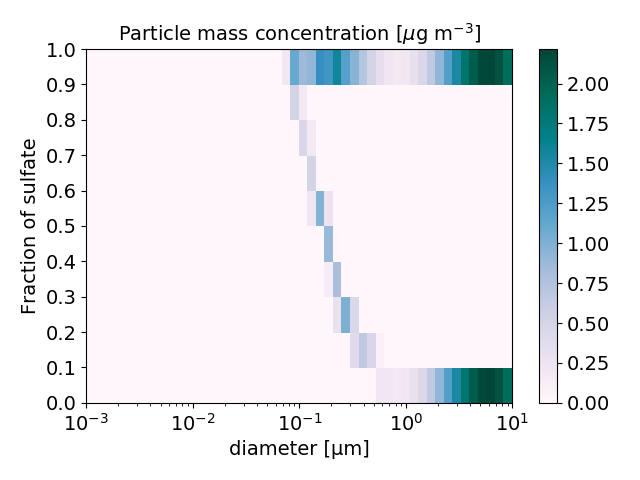
\includegraphics[angle=0,width=0.45\textwidth]{../graph/figure_ref/cond_mass_ext_out.png}
        \end{center}
\caption{Mass concentrations as a function of the size and fraction of one of the
two compounds at initial time (left panel) and after 12 h of simulation (right panel).}
\label{fig-cond-extb}
\end{figure}
 
\subsection{Viscosity}
     
The gas/particle mass transfer is strongly affected by particle viscosity. To
illustrate this effect, the condensation of hydrophobic organic surrogates of different volatility is studied for different
values of the viscosity, represented by different values of the organic-phase
diffusion coefficients D (10$^{-18}$, 10$^{-19}$, 10$^{-20}$,
10$^{-21}$, 10$^{-22}$, 10$^{-23}$, 10$^{-24}$ m$^2$~s$^{-1}$). The value
D~=~10$^{-12}$ m$^2$~s$^{-1}$ corresponds to an inviscid particle, while the value
D~=~10$^{-24}$ m$^2$~s$^{-1}$ corresponds to a very viscous particle.
Each particle is discretized into 5 layers to model the flux of diffusion of the
organic compounds in the particle. 
The test cases presented here are similar to those of the Figure 6 of \cite{couvidat2015}. 
Three surrogates are successively studied: SOAlP, POAlP and POAmP and  which have 
 partitioning coefficients K$_p$ equal to 100~m$^3$~$\mu$g$^{-1}$,
 1~m$^3$~$\mu$g$^{-1}$, and 0.01~m$^3$~$\mu$g$^{-1}$.
The surrogate that condenses is initially only in the gas
phase, with a mass of 5 $\mu$g~m$^{-3}$. It condenses on an organic phase of
5~$\mu$g~m$^{-3}$ made of SOAlP, which has a very low volatility (K$_p$~=~100~m$^3$~$\mu$g$^{-1}$).
The test cases may be launched by launching the script
 {\it{INIT/launch\_visco.sh}}. After computation of the condensation of the surrogates
from different values of the viscosity, three graphs can be displayed by
running the scripts {\it{conc\_visco\_poalp.py}}, {\it{conc\_visco\_poamp.py}},
{\it{conc\_visco\_soalp.py}} (one graph per surrogate). They are shown in 
Fig~\ref{fig-visco}, which represents the time variations of particle-phase organic
concentrations of the surrogate (POAlP in upper left panel, POAmP in upper
right panel and SOAlP in lower panel). 
The surrogate of low volatility (SOAlP) condenses quickly onto the organic
phase, independently of the viscosity (upper left panel of Fig~\ref{fig-visco}). All the organic mass is then in the
particle phase.  
Although the condensation of POAlP is influenced by the viscosity, a large fraction of the gas-phase concentration of POAlP condenses quickly (upper right panel of Fig~\ref{fig-visco}).
For POAmP, which is the most volatile of the three surrogates, high viscosity
(low diffusion coefficient) strongly inhibits the condensation of POAmP (lower right panel of Fig~\ref{fig-visco}).

\begin{figure}[H]
        \begin{center}
                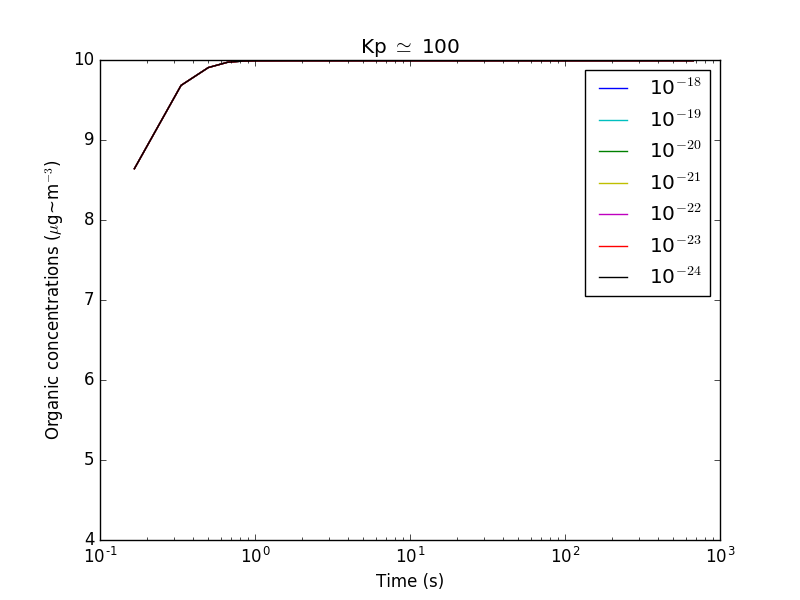
\includegraphics[angle=0,width=0.45\textwidth]{../graph/figure_ref/visco_soalp.png}
                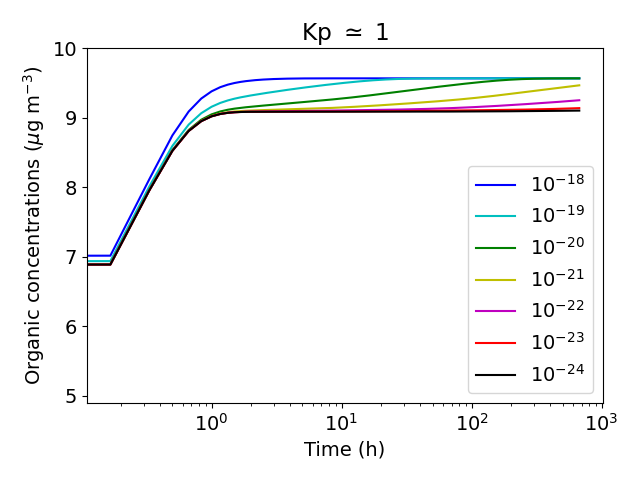
\includegraphics[angle=0,width=0.45\textwidth]{../graph/figure_ref/visco_poalp.png}
                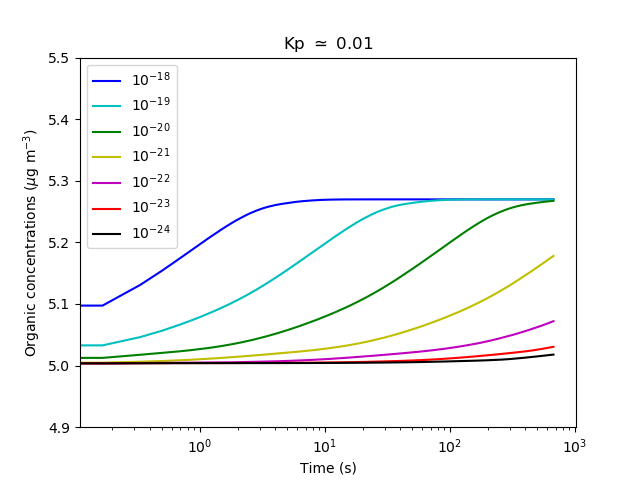
\includegraphics[angle=0,width=0.45\textwidth]{../graph/figure_ref/visco_poamp.png}
        \end{center}
\caption{Viscosity test case: time evolution of organic concentrations (SOAlP
  in the upper left, POAlP in the upper right, POAmP in the lower left) for
  several organic-phase diffusivity: 10$^{-18}$ (dark blue), 10$^{-19}$ (light
  blue), 10$^{-20}$ (green), 10$^{-21}$ (yellow),
10$^{-22}$ (magenta), 10$^{-23}$ (red), 10$^{-24}$ (black) m$^2$~s$^{-1}$.}
\label{fig-visco}
\end{figure}
       
\bigskip

\section{References}
%\addcontentsline{toc}{section}{References}
\bibliographystyle{apalike}
\bibliography{testcases}

\end{document}
